%%
%% Author: mirco
%% 19.06.18
%%

% Preamble
\documentclass[11pt,aspectratio=169,usenames,dvipsnames]{beamer}
%\documentclass[11pt,aspectratio=169,usenames,dvipsnames,handout]{beamer}
\usepackage[english]{babel}
\usepackage{blindtext}
\usepackage{tabularx,booktabs}
\usetheme{Copenhagen}
%\usecolortheme{crane}
\usepackage[autostyle]{csquotes}
\usepackage{graphicx}
\usepackage{amsmath}
\setbeamertemplate{navigation symbols}{}
\usepackage{nicefrac}
\usepackage{framed}
\setbeamercovered{transparent}
\setbeamertemplate{section page}
{
\begin{centering}
    \begin{beamercolorbox}[sep=12pt,center]{part title}
        \usebeamerfont{section title}\insertsection\par
    \end{beamercolorbox}
\end{centering}
}
%\usepackage{beamerthemeshadow}

\setbeamertemplate{subsection page}
{
\begin{centering}
    % \begin{beamercolorbox}[sep=5pt,center]{part title}
    \par
    \usebeamerfont{section title}\insertsubsection\par
    %  \end{beamercolorbox}
\end{centering}
}


\title{Comparative Argument Mining}
\author{Mirco Franzek}
\date{June 26, 2018}
\begin{document}
    \maketitle

    \section{Introduction}
    \frame{\sectionpage}

    \begin{frame}[t]
        \frametitle{Comparative Argument Mining: An example}
        Given a sentence and two comparable objects like:

        \begin{center}
            \LARGE \enquote{\textcolor{orange}{Toyota} is better than \textcolor{RoyalBlue}{BMW} at\ldots providing reliable, economical auto transport.}
        \end{center}
        \pause
        we want to know if
        \begin{itemize}
            \item the sentence compares \textcolor{orange}{the first object} and \textcolor{RoyalBlue}{the second object}   \pause
            \item \textcolor{orange}{the first object} wins the comparison or   \pause
            \item \textcolor{RoyalBlue}{the second object} wins the comparison
        \end{itemize}

    \end{frame}

    \begin{frame}[t]
        \frametitle{Related Work}
        \begin{itemize}
            \item Little work on comparative argument mining
            \item Specific to a narrow domain, e.g. drug therapy
            \item See \cite{fiszman2007interpreting}, \cite{Park:2012:ICC:2391171.2391173} and \cite{gupta2017identifying}
            \item Patterns and rule based systems
        \end{itemize}

    \end{frame}


    \section{Creating a data set}
    \frame{\sectionpage}
    \subsection{Data Source}
    \frame{\subsectionpage}

    \begin{frame}[t]
        \frametitle{Needed Data}
        English sentences
                \begin{enumerate}
            \item with a high chance of being comparative
            \item containing at least two comparable objects\\
            \begin{scriptsize}
                (Not like: \enquote{\textcolor{ForestGreen}{This} is better than \textcolor{RoyalBlue}{BMW} \ldots})
            \end{scriptsize}
        \end{enumerate}\pause

        Objects, which are
        \begin{enumerate}
            \item comparable on at least one property
            \item known by many people
        \end{enumerate}\pause
        Everything should be as domain unspecific as possible.
    \end{frame}

    \begin{frame}[t]
        \frametitle{English sentences: CommonCrawl}
        \begin{itemize}
            \item CommonCrawl\footnote{\url{http://commoncrawl.org}} is a freely accessible data set of crawled websites
            \item A preprocessed version\footnote{\cite{Panchenko:2017aa}} was used
            \begin{itemize}
                \item HTML was removed
                \item Splitted into sentences
                \item Duplicates were removed
            \end{itemize}\pause
            \item 3,288,963,864 unique sentences; inserted into an Elasticsearch index
            \item Comparisons: 428,932 sentences contain \enquote{is better than}
        \end{itemize}

    \end{frame}

    \begin{frame}[t]
        \frametitle{Objects and Domains}
        \begin{itemize}
            \item The objects were taken from three domains:
            \begin{enumerate}
            \item \textbf{Computer Science}: operating systems, abstract concepts, software, \ldots
            \item \textbf{Brands}: cars, food, electronics, \ldots
            \item \textbf{Random}: book authors, soccer teams, universities, \ldots
            \end{enumerate}
            \item 271 pairs in total

        \end{itemize}
    \end{frame}

    \begin{frame}[t]
        \frametitle{Obtaining objects}
        \begin{itemize}
            \item Wikipedia's \enquote{List of \ldots} pages were used to select suitable objects for Computer Science and Brands.\pause
            \item Random
            \begin{itemize}
                \item 25 seed words were randomly selected (e.g. cork, Hamster, Florida, ninja\ldots)
                \item JoBimText\footnote{http://ltmaggie.informatik.uni-hamburg.de/jobimtext/} was used to find the 10 most similar words for each seed word
            \end{itemize}\pause
            \item Each object was checked against a frequency dictionary.
            \item Objects with a frequency of zero were removed.
            \item All possible combinations for each object type (Wikipedia page or seed word) were created.
        \end{itemize}

    \end{frame}

    \begin{frame}[t]
        \frametitle{Pairs: Examples}

        \begin{tabularx}{\textwidth}{XXX}
            \toprule
            Brands & Computer Science & Random \\
            \midrule
            Microsoft vs. Apple & Java vs. Python & baseball vs. hockey \\
            Nikon vs. Leica & Eclipse vs. Netbeans & fishing vs. swimming\\
            Coca-Cola vs. Pepsi & OpenGL vs. Direct3D & SUV vs. minivan\\
            Nike vs. Adidas & Integer vs. Float & Kennedy vs. Nixon\\
            Ibuprofen vs. Advil & USB vs. Bluetooth & plastic vs. wood\\
            Ford vs. Honda & Oracle vs. MysQL & Harvard vs. Princeton\\

            \bottomrule

        \end{tabularx}

    \end{frame}

    \begin{frame}[t]
        \frametitle{Sentence Sampling}

        \begin{itemize}
            \item 21 words (e.g. better, worse, slower, inferior, cooler) were selected as \textbf{cue words} for comparisons\pause
            \item for 90 percent of the pairs, the index was queried for sentences containing both objects of the pair and at least one cue word
            \item the cue word was omitted for the remaining 10 percent\pause
            \item 2500 sentences for each domain were randomly sampled from the result
        \end{itemize}

    \end{frame}

    \begin{frame}[t]
        \frametitle{Sentence Sampling: Examples}
        \begin{enumerate}
            \item \enquote{There is no doubt \textcolor{orange}{Python} is better than \textcolor{RoyalBlue}{Ruby} at any in aspect you will pick.}
            \item \enquote{Goodnight \textcolor{orange}{NetBeans}, Hello \textcolor{RoyalBlue}{Eclipse}}
            \item \enquote{\textcolor{orange}{stone} is harder than \textcolor{RoyalBlue}{metal}}
            \item \enquote{arrrggghh...\textcolor{orange}{Python} is a terrible language - only \textcolor{RoyalBlue}{Perl} sucks worse.}
            \item \enquote{Good to see again a \textcolor{orange}{Renault} ahead of a \textcolor{RoyalBlue}{Ferrari}.}
        \end{enumerate}
    \end{frame}

    \subsection{Crowdsourcing}
    \frame{\subsectionpage}
    \begin{frame}[t]
        \frametitle{Task Design}
        \begin{itemize}
            \item All sentences were annotated via the crowdsourcing platform Crowdflower\footnote{\url{https://crowdflower.com}}.
            \item A prestudy was conducted to assess the quality of the annotation guidelines and the sentence selection process.
            \item About 25 percent were labeled as comparative in the prestudy.
            \item Each sentence was annotated by at least five annotators.
        \end{itemize}

    \end{frame}

    \begin{frame}[t]
        \frametitle{Task Design: Problems}
        Initially, the annotators were asked to answer the question:
        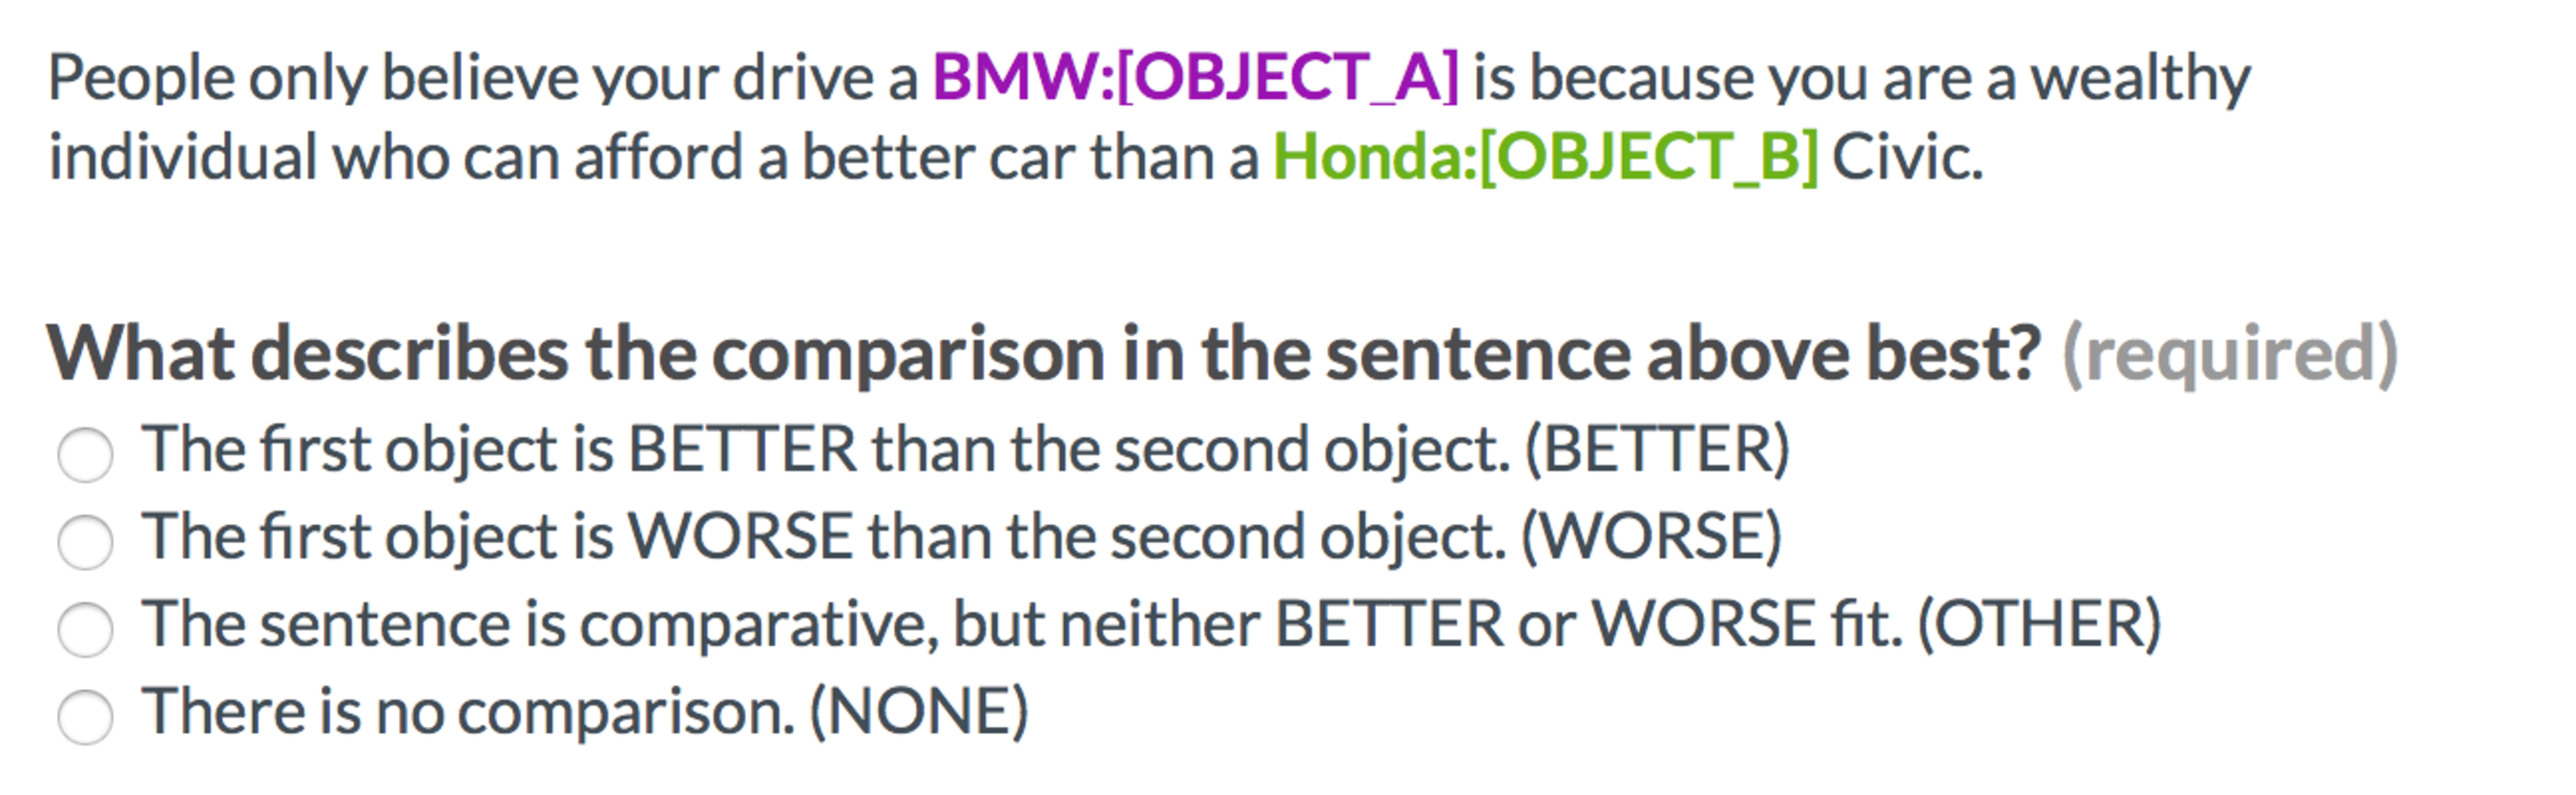
\includegraphics[scale=0.3]{images/q1other}
    \end{frame}


    \begin{frame}[t]
        \frametitle{Task Design: Problems}
        \only<1-2>{
        \begin{itemize}
            \item People confused \texttt{OTHER} with \texttt{NONE} frequently.
            \item People were dissatisfied because the choice between the two labels was too difficult.\pause
                   \item \texttt{OTHER} and \texttt{NONE} were hardly distinguishable in first classification experiments.

            \item After 750 annotated sentences per domain, \texttt{OTHER} was dropped.
                 \item \texttt{OTHER} was merged into \texttt{NONE} for the classification experiments.
        \end{itemize}
        }

        \only<3>{
        \begin{itemize}
            \item The annotation guidelines stated that all questions should be labelled as \texttt{NONE}.
            \begin{scriptsize}
                (For instance, \enquote{Is \textcolor{orange}{Python} better than \textcolor{RoyalBlue}{Ruby}?})
            \end{scriptsize}
            \item This was frequently overlooked by the annotators.
        \end{itemize}
        }
    \end{frame}




    \begin{frame}
        \frametitle{Results: Brands}
        \begin{columns}
            \column{2in}
            \begin{itemize}
                \item 2335 sentences in total
                \item 571 comparative sentences (24 percent)
            \end{itemize}
            \column{3in}
            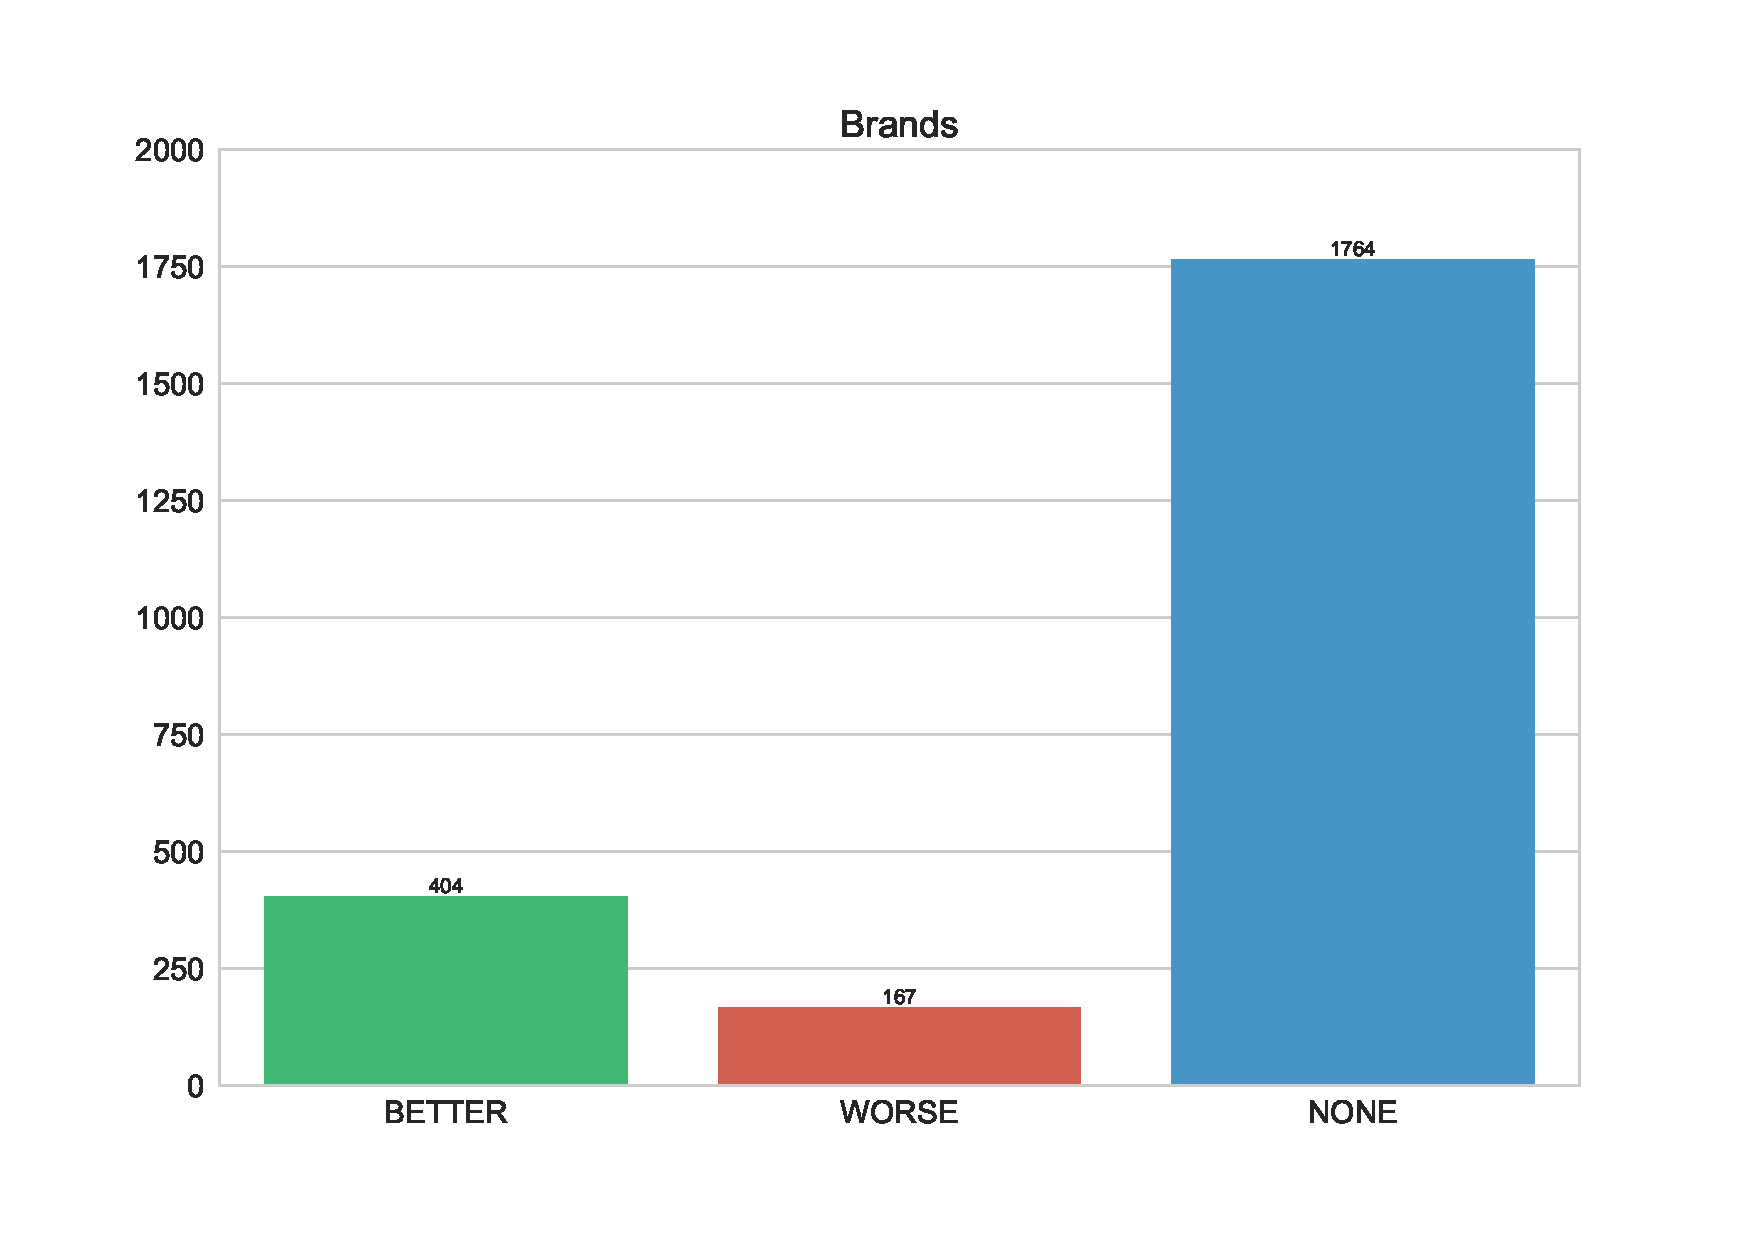
\includegraphics[scale=0.45,trim={1cm 0 2cm 1cm},clip]{images/Brands-dist}
        \end{columns}
    \end{frame}

    \begin{frame}[t]
        \frametitle{Results: Computer Science}
        \begin{columns}
            \column{2in}
            \begin{itemize}
                \item 2425 sentences in total
                \item 829 comparative sentences (34 percent)
            \end{itemize}
            \column{3in}
            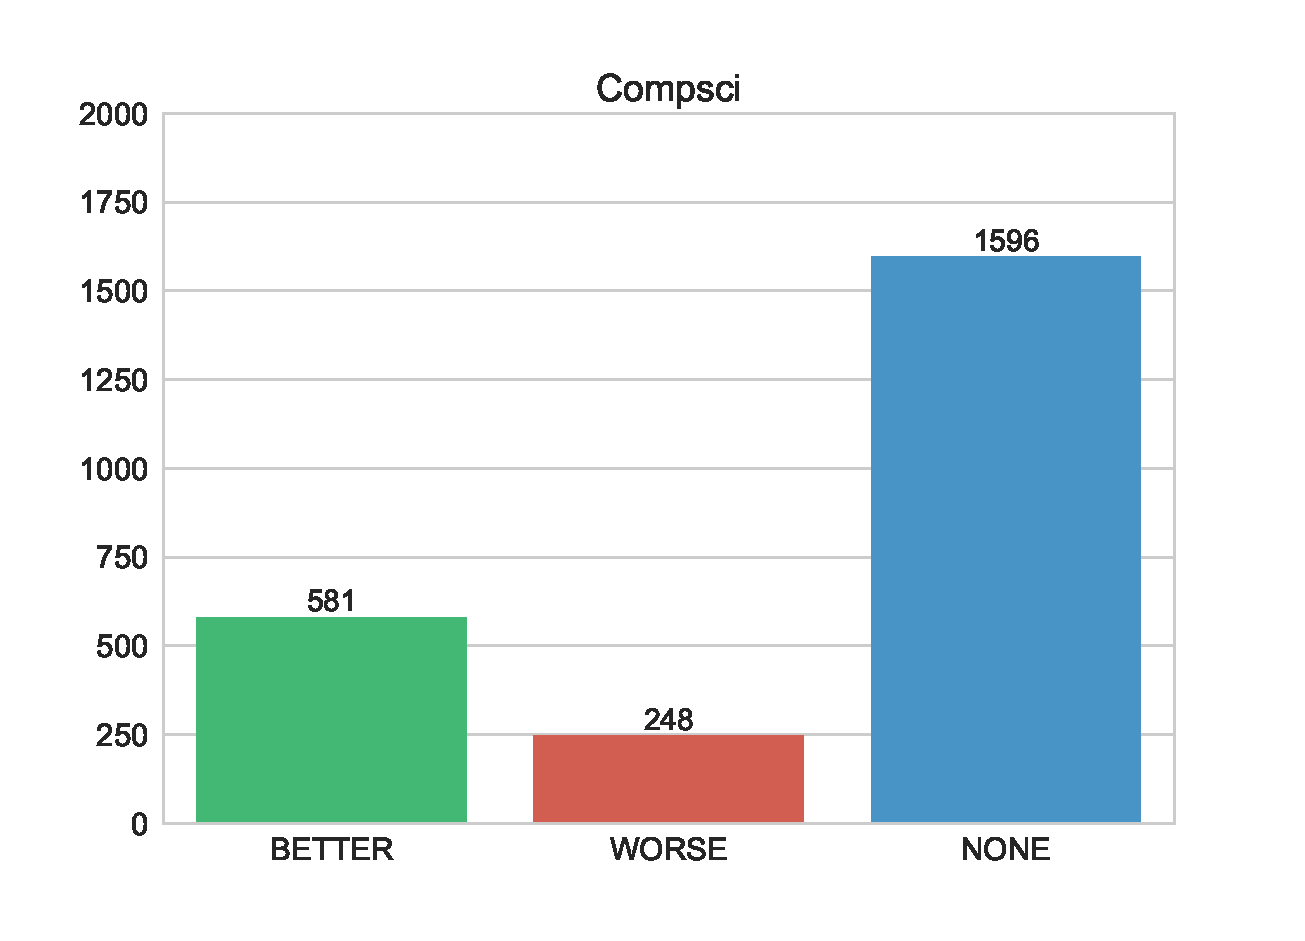
\includegraphics[scale=0.45,trim={1cm 0 2cm 1cm},clip]{images/Compsci-dist.pdf}
        \end{columns}
    \end{frame}

    \begin{frame}[t]
        \frametitle{Results: Random}
        \begin{columns}
            \column{2in}
            \begin{itemize}
                \item 2439 sentences in total
                \item 557 comparative sentences (22 percent)
            \end{itemize}
            \column{3in}
            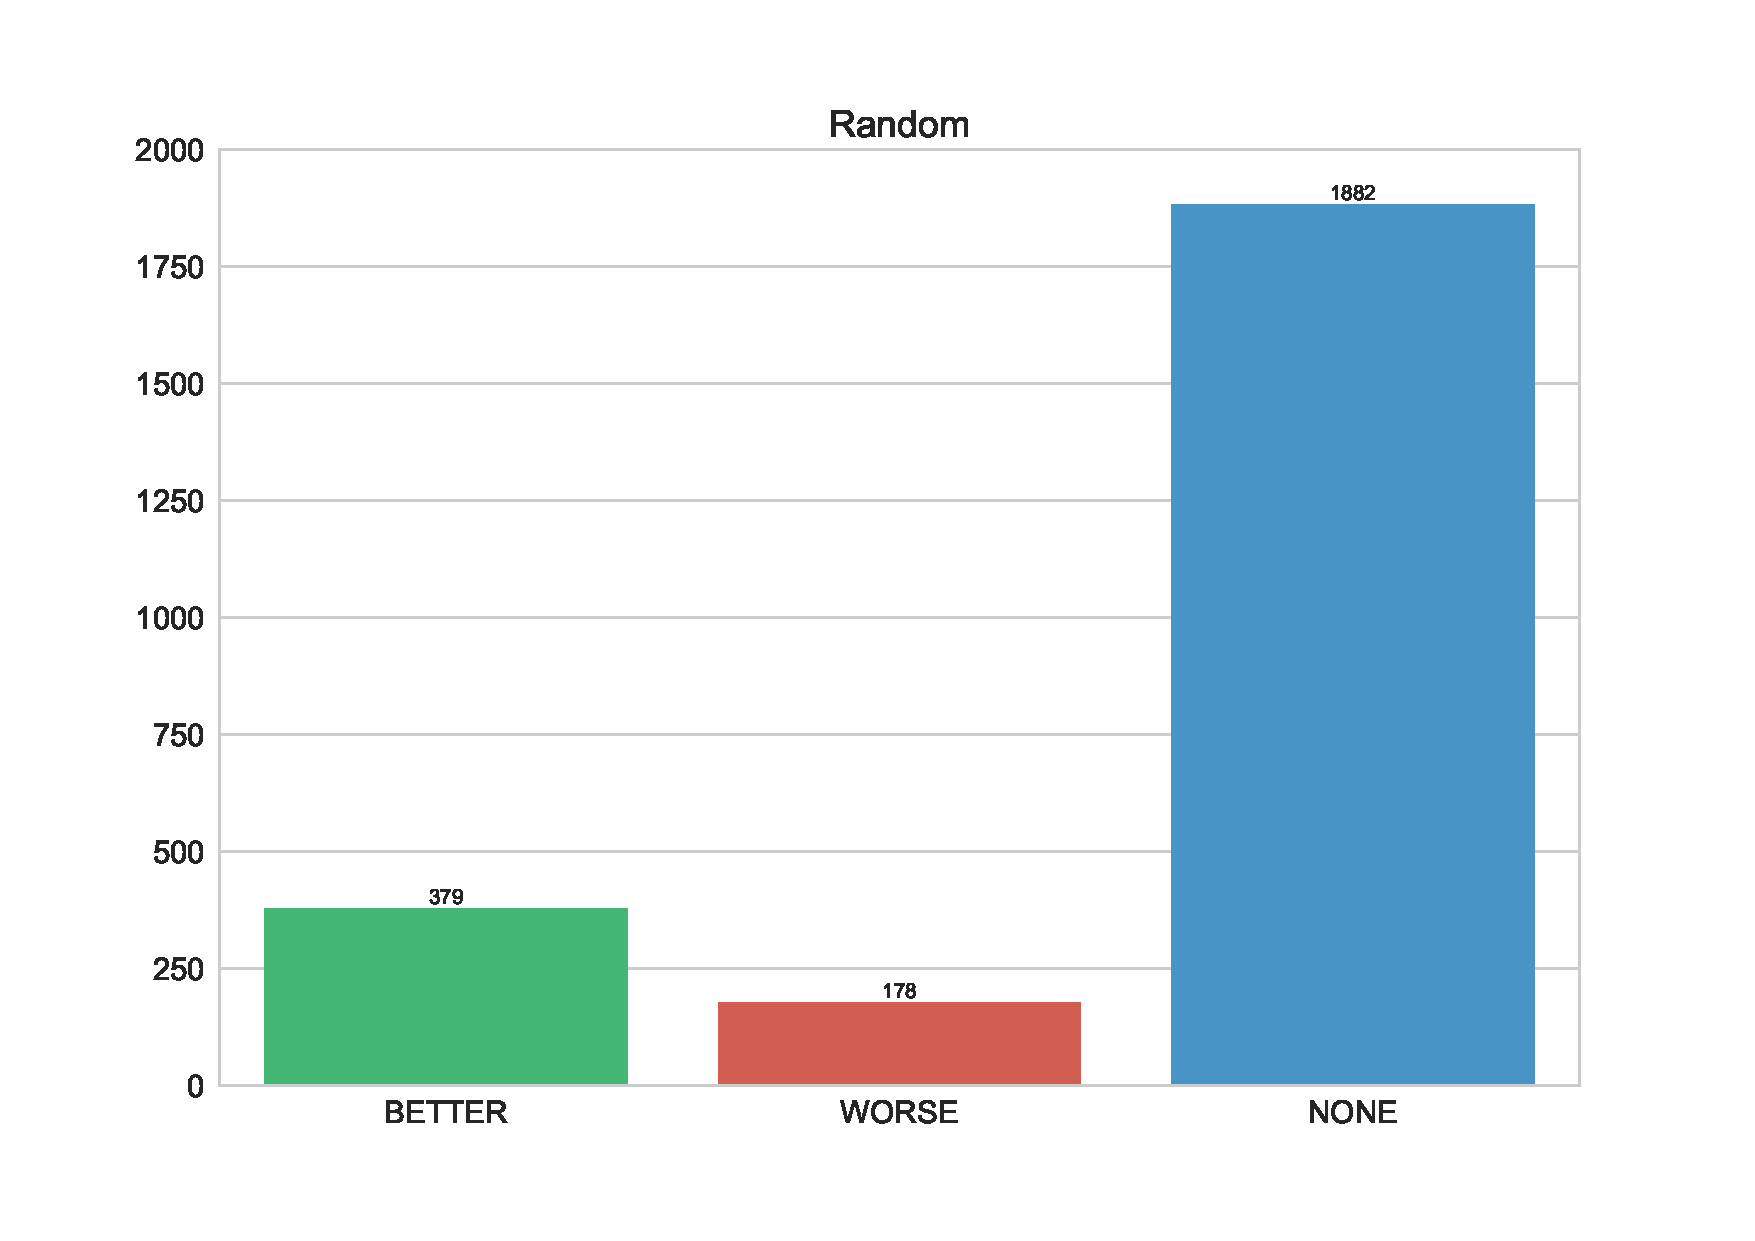
\includegraphics[scale=0.45,trim={1cm 0 2cm 1cm},clip]{images/Random-dist.pdf}
        \end{columns}
    \end{frame}

    \begin{frame}[t]
        \frametitle{Results: All Domains}
        \begin{columns}
            \column{2in}
            \begin{itemize}
                \item 7199 sentences in total
                \item 1957 comparative sentences (27 percent)
                \item the class \texttt{BETTER} is more than two times bigger than \texttt{WORSE}
            \end{itemize}
            \column{3in}
            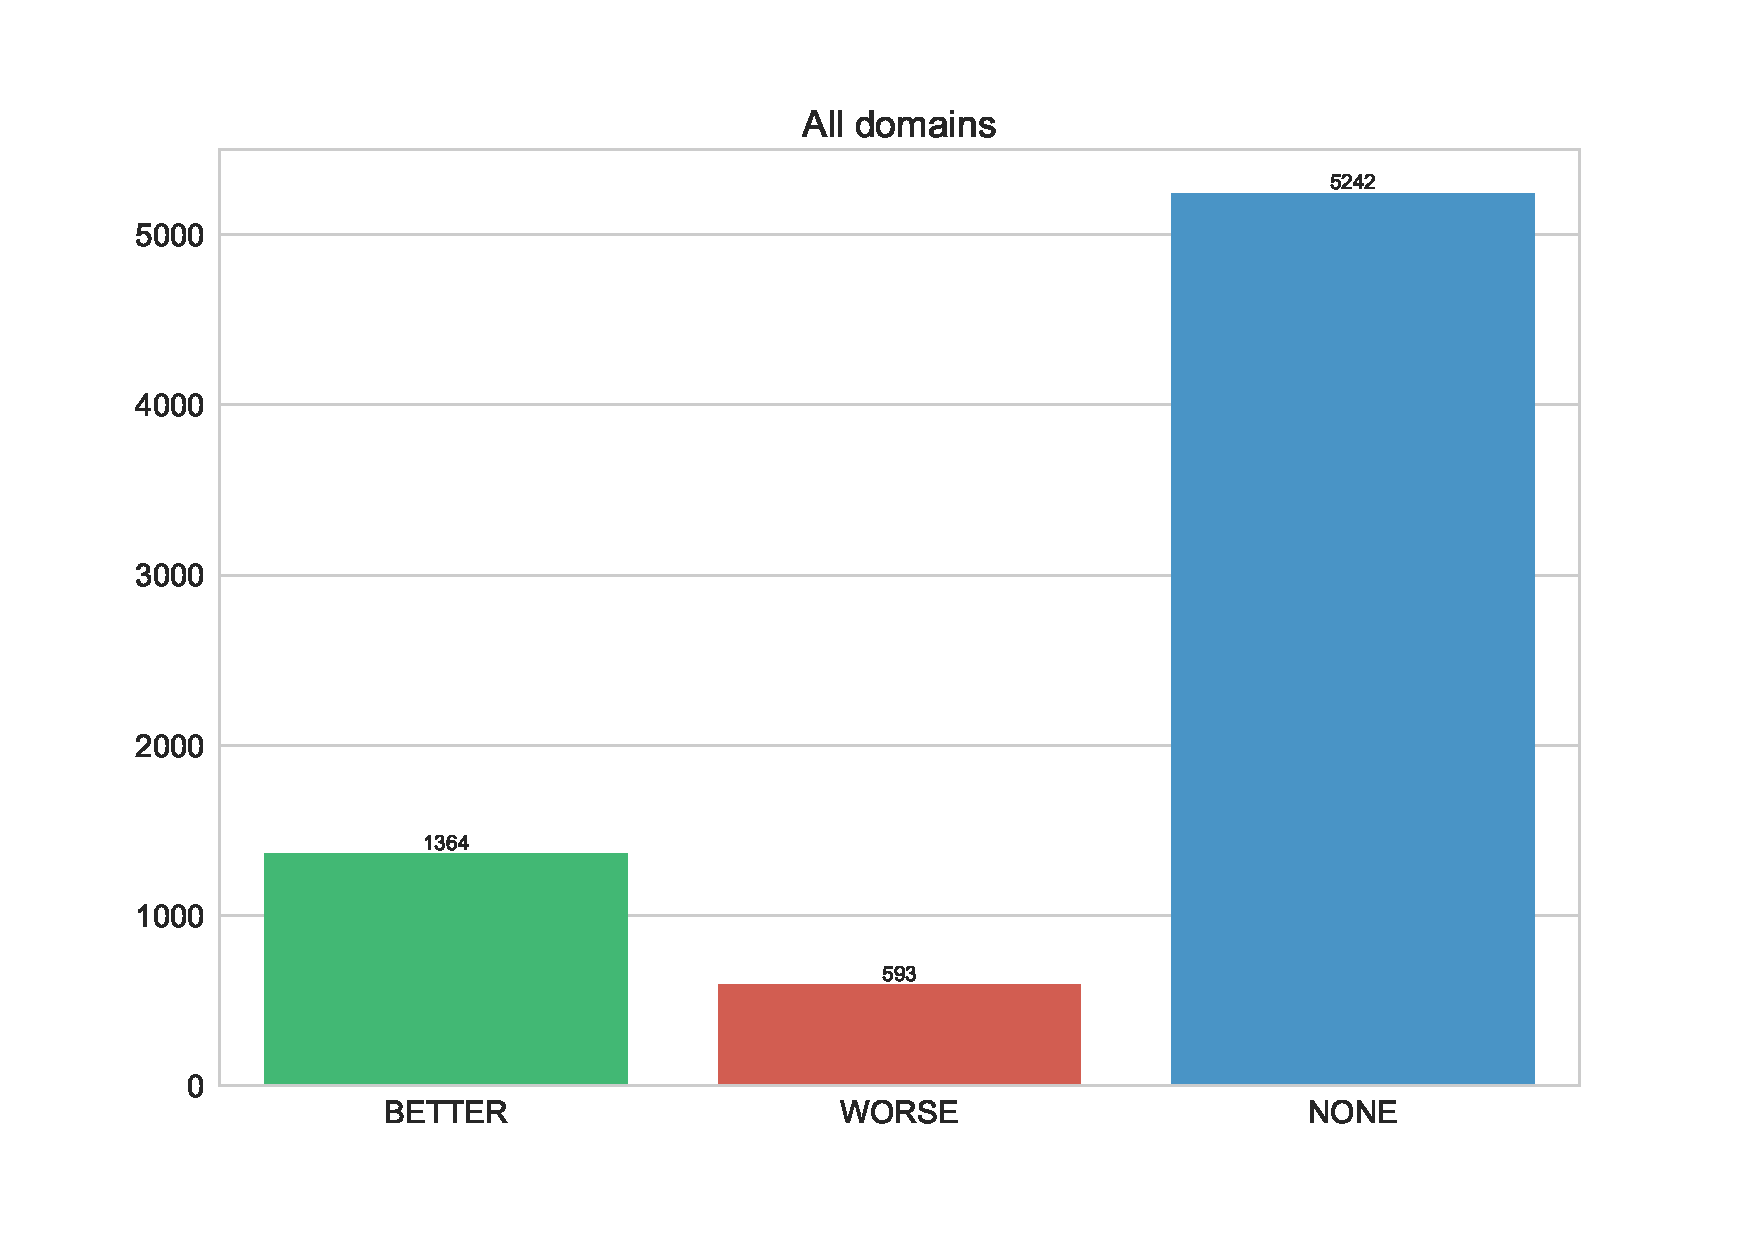
\includegraphics[scale=0.45,trim={1cm 0 2cm 1cm},clip]{images/Alldomains-dist.pdf}
        \end{columns}
    \end{frame}

    \begin{frame}[t]
        \frametitle{Results: All Domains}



        \begin{columns}
            \column{2in}
            \begin{itemize}
                \item 7199 sentences in total
                \item 1957 comparative sentences (27 percent)
                \item the class \texttt{BETTER} is more than two times bigger than \texttt{WORSE}
            \end{itemize}
            \column{3in}
            Annotation confidence for all domains. The confidence is calculated as $\nicefrac{\text{judgments for majority class}}{\text{total judgments}}$.
            \begin{tabular}{@{}rrr@{}}
                \toprule
                Confidence & Sentences & \% of data set \\
                \midrule
                100\%    & 5111 & 71.00     \\
                91-99\%    & 0 & 0.00     \\
                81-90\%    & 75 & 1.04     \\
                71-80\%    & 1057 & 14.68     \\
                61-70\%    & 33 & 0.46     \\
                51-60\%    & 754 & 10.47     \\
                0-50\%    & 169 & 2.35     \\
                \bottomrule
            \end{tabular}

        \end{columns}


    \end{frame}


    \section{Classification}
        \frame{\sectionpage}
    
    \subsection{Setup}
    \frame{\subsectionpage}

    
    
        \begin{frame}[t]
        \frametitle{Setup}
        \begin{itemize}
            \item The 7199 sentences were split into a development (5759) and held-out (1440) set.
            \item All experiments were conducted on the development set and evalutated with k-folds cross validation ($k = 5$)\pause
            \item Two setups: 
            \begin{enumerate}
            \item \textbf{Three classes}: \texttt{NONE}, \texttt{BETTER} and \texttt{WORSE}
            \item\textbf{Binary}: \texttt{NONE} and \texttt{ARG} (= \texttt{BETTER} $\cup$ \texttt{WORSE})
            \end{enumerate}
        \end{itemize}

    \end{frame}

    
    
    \begin{frame}[t]
        \frametitle{Algorithms}
        \begin{columns}[t]
            \column{2in}
            \begin{itemize}
                \item 13 classification algorithms were tested with a bag-of-words-model
              \item XGBoost with 1000 base estimators was used in all experiments
                         \begin{scriptsize}
                    (gradient boosted decision trees; presented in \cite{DBLP:journals/corr/ChenG16})
                \end{scriptsize}
                          \item  The graphic shows the f1 score and standard derivation (black bar).
            \end{itemize}
            \column{3.5in}

            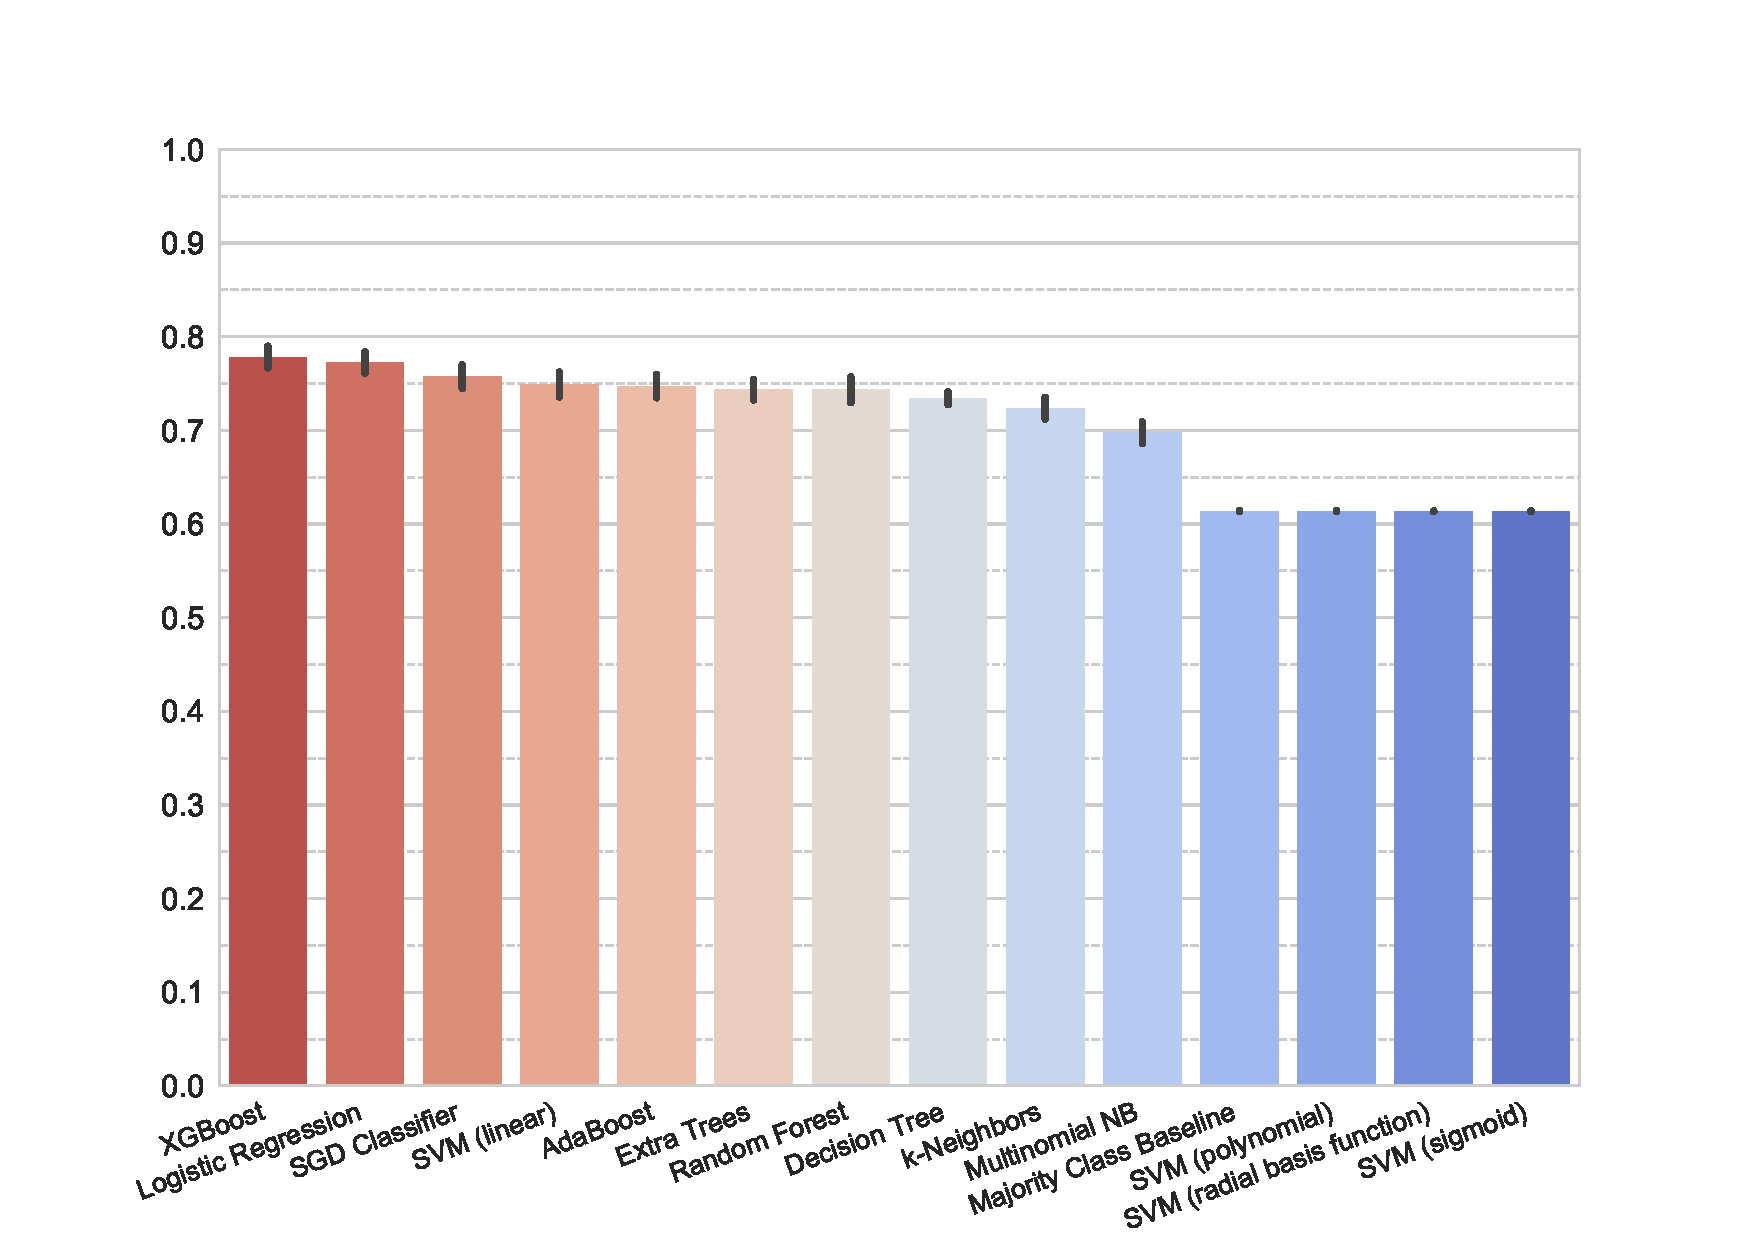
\includegraphics[scale=0.35,trim={1cm 0 0 5.45cm},clip]{images/classifier.pdf}


        \end{columns}
    \end{frame}


    \begin{frame}[t]
        \frametitle{Baseline: Three classes}

        \begin{minipage}{.5\linewidth}
            \label{tbl:3stratifiedbaseline}
            \centering
            Random (stratified) baseline\newline\newline
            \begin{tabularx}{0.97\linewidth}{Xrrrr}
                \toprule
                & precision & recall & f1 score                     \\ \midrule
                \texttt{B} & 0.19 \scriptsize{$\pm$0.01} & 0.21 \scriptsize{$\pm$0.01} & 0.20 \scriptsize{$\pm$0.01} \\
                \texttt{W}  & 0.06 \scriptsize{$\pm$0.02} & 0.05 \scriptsize{$\pm$0.02} & 0.06 \scriptsize{$\pm$0.03} \\
                \texttt{N}   & 0.73 \scriptsize{$\pm$0.00}  & 0.73 \scriptsize{$\pm$0.00} & 0.73 \scriptsize{$\pm$0.00} \\
                avg. & 0.57 \scriptsize{$\pm$0.00} & 0.58 \scriptsize{$\pm$0.01} & 0.57 \scriptsize{$\pm$0.00} \\
                \bottomrule
            \end{tabularx}

        \end{minipage}%
        \begin{minipage}{.5\linewidth}
            \centering
            Most frequent class baseline\newline\newline
            \begin{tabularx}{0.97\linewidth}{Xrrrr}
                \toprule
                & precision & recall & f1 score                                    \\ \midrule
                \texttt{B} & 0.00 \scriptsize{$\pm$0.00} & 0.00 \scriptsize{$\pm$0.00} & 0.00 \scriptsize{$\pm$0.00}                \\
                \texttt{W}  & 0.00 \scriptsize{$\pm$0.00} & 0.00 \scriptsize{$\pm$0.00} & 0.00 \scriptsize{$\pm$0.00}                \\
                \texttt{N}   & 0.73 \scriptsize{$\pm$0.00}     & 1.00 \scriptsize{$\pm$0.00} & 0.84 \scriptsize{$\pm$0.00}                \\
                avg. & 0.53 \scriptsize{$\pm$0.00} & 0.73 \scriptsize{$\pm$0.00} & \textbf{0.61} \scriptsize{$\pm$0.00} \\
                \bottomrule
            \end{tabularx}
        \end{minipage}\newline\newline
        \texttt{B} = \texttt{BETTER}, \texttt{W} = \texttt{WORSE}, \texttt{N} = \texttt{NONE},
    \end{frame}

    \begin{frame}[t]
        \frametitle{Baseline: Binary}


        \begin{minipage}{.5\linewidth}

            \centering
            Random (stratified) baseline\newline\newline
            \begin{tabularx}{0.97\linewidth}{Xrrrr}
                \toprule
                & precision & recall & f1 score                              \\ \midrule
                \texttt{ARG}  & 0.26 \scriptsize{$\pm$0.03} & 0.26 \scriptsize{$\pm$0.03} & 0.26 \scriptsize{$\pm$0.03}          \\
                \texttt{N} & 0.72 \scriptsize{$\pm$0.01} & 0.72 \scriptsize{$\pm$0.01} & 0.72 \scriptsize{$\pm$0.01}          \\
                avg. & 0.60 \scriptsize{$\pm$0.02} & 0.60 \scriptsize{$\pm$0.02} & 0.60 \scriptsize{$\pm$0.02} \\
                \bottomrule
            \end{tabularx}

        \end{minipage}%
        \begin{minipage}{.5\linewidth}
            \centering
            Most frequent class baseline\newline\newline
            \begin{tabularx}{0.97\linewidth}{Xrrrr}
                \toprule
                & precision & recall & f1 score                     \\ \midrule
                \texttt{ARG}  & 0.00 \scriptsize{$\pm$0.00} & 0.00 \scriptsize{$\pm$0.00} & 0.00 \scriptsize{$\pm$0.00} \\
                \texttt{N} & 0.73 \scriptsize{$\pm$0.00} & 1.00 \scriptsize{$\pm$0.00} & 0.84 \scriptsize{$\pm$0.00} \\
                avg. & 0.53 \scriptsize{$\pm$0.00} & 0.73 \scriptsize{$\pm$0.00} & \textbf{0.61} \scriptsize{$\pm$0.00} \\
                \bottomrule
            \end{tabularx}
        \end{minipage}\newline\newline
        \texttt{ARG} = \texttt{BETTER} + \texttt{WORSE}, \texttt{N} = \texttt{NONE}


    \end{frame}

    \subsection{Features}
    \frame{\subsectionpage}
    
    
    \begin{frame}[t]
        \frametitle{Feature Overview}
        \begin{itemize}
            \item Bag-of-words
            \item 500 most frequent part-of-speech bi-, tri and four-grams
            \item Mean word embedding vector (GloVe vectors, size 300)
            \item A boolean feature capturing the appearance of a comparative adjective (Contains JJR)
            \item Sentence Embeddings
            \item Dependency Paths
        \end{itemize}
      
    \end{frame}
    
    \begin{frame}[t]
        \frametitle{Sentence Embeddings}
        \begin{itemize}
            \item Dense vector representation for phrases, similar to word embeddings\pause
            \item Several approaches, for instance SkipThrough \cite{NIPS2015_5950}, Paragraph Vectors \cite{Le:2014aa} and \textbf{InferSent} \cite{Conneau:2017aa}
            \item A pretrained InferSent model\footnote{https://github.com/facebookresearch/InferSent} was used in the thesis
        \end{itemize}


    \end{frame}

    \begin{frame}[t]
        \begin{columns}
            \column{2.8in}
            \begin{itemize}
                \item<1-> Neural Network trained on the Stanford Natural Language Inference (SNLI) corpus
                \item<1-> SNLI contains 570k sentence pairs labelled as contradiction, entailment or neutral
                \item<2-> BiLSTM with max-pooling and 4096 neurons as encoders
                \item<2-> tested on a wide range of tasks
                \item<2->  outperforms SkipThrough and Paragraph Vectors
            \end{itemize}
            \column{3in}
            \only<1->{
            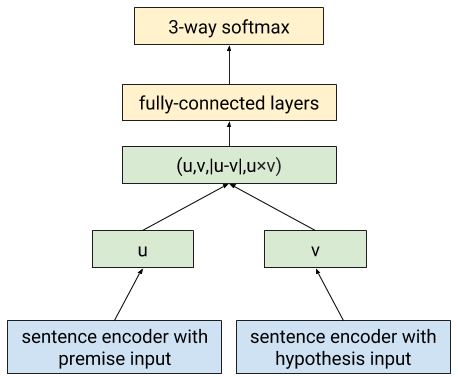
\includegraphics[scale=0.5,trim={0cm 0 0cm 0cm},clip]{images/nli}}
        \end{columns}
    \end{frame}

    \begin{frame}[t]
        \frametitle{HypeNet and LexNet}
        \begin{itemize}
            \item HypeNet\footnote{\cite{DBLP:conf/acl/ShwartzGD16}} combines word embeddings and (dependency) path-based information to check if two words are hypernyms.
            \item LexNet\footnote{\cite{DBLP:journals/corr/ShwartzD16}} is a generalization of HypeNet to find multiple semantic relations.\pause
            \item HypeNet creates a string representation of the dependency path between two words
            \item The string representations are then encoded using an LSTM.
            \item The average of all paths for each word pair is used as the path feature.
        \end{itemize}
    \end{frame}


    \begin{frame}[t]
        \frametitle{HypeNet and LexNet: Example}
        \begin{center}
            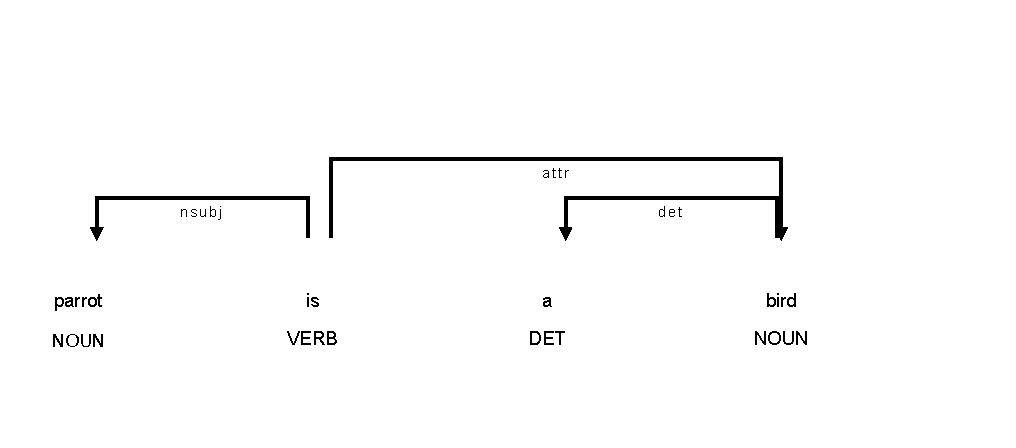
\includegraphics[scale=0.7,trim={0cm 0.5cm 0cm 0.25cm},clip]{images/hypenet_example}
        \end{center}

        \begin{itemize}
            \item \texttt{X/NOUN/nsubj/< be/VERB/ROOT/- Y/NOUN/attr/>}
            \item Each node contains lemma, part of speech, dependency label and the edge direction.
            \item Expectation: path embeddings add valuable information to sentence embeddings.

        \end{itemize}
    \end{frame}


    \begin{frame}[t]
        \frametitle{HypeNet and LexNet: Features}
        \begin{itemize}
            \item Two features based on HypeNet paths:\pause
            \item \textbf{LexNet (original)} creates paths as described in the paper
            \begin{itemize}
                \item maximum length of four
                \item the first object must be reachable from following only left edges, starting from the lowest common head
                \item the second object must be reachable from following only right edges 
                \item 1519 sentences without a path\pause
            \end{itemize}
            \item \textbf{LexNet (optimized)}
            \begin{itemize}
                \item maximum length of sixteen
                \item no restrictions on the direction
                \item 399 sentences without a path
            \end{itemize}
        \end{itemize}
    \end{frame}





    
    \begin{frame}[t]
    \frametitle{Preprocessing}
    Selection of the sentence part
        \begin{itemize}
    \item the whole sentence
    \item all words between the first and the second object
    \item all words before the first object
    \item all words after the second object\pause
    \end{itemize}
    Object replacement
    \begin{itemize}
    \item leave the objects
    \item remove both objects
    \item replace both objects with the term \texttt{OBJECT}
    \item replace the first object with \texttt{OBJECT\_A} and the second with \texttt{OBJECT\_B} 
    \end{itemize}
    


    \end{frame}


    \subsection{Training Results}
    \frame{\subsectionpage}
    \begin{frame}[t]
        \frametitle{Three classes: F1 score}
        \centerline{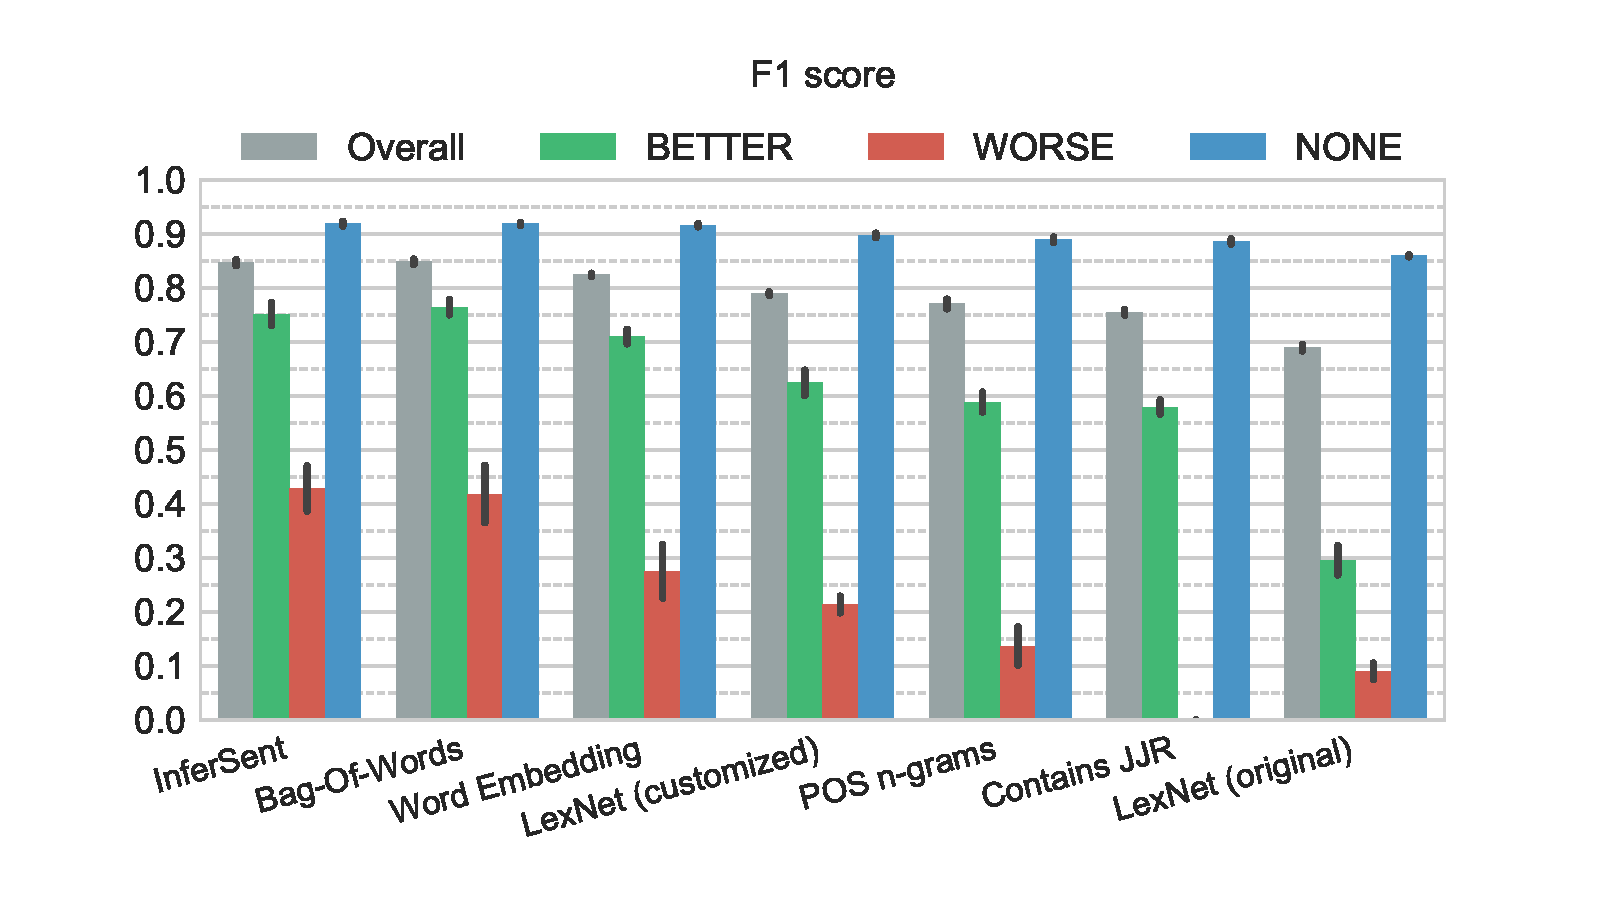
\includegraphics[scale=0.45,trim={0 0 0 0.5cm},clip]{images/experiments/p-f1-False}}
    \end{frame}


    \begin{frame}[t]
        \frametitle{Three classes: Precision and Recall}
        \begin{columns}[t]
            \column{2in}
            \centerline{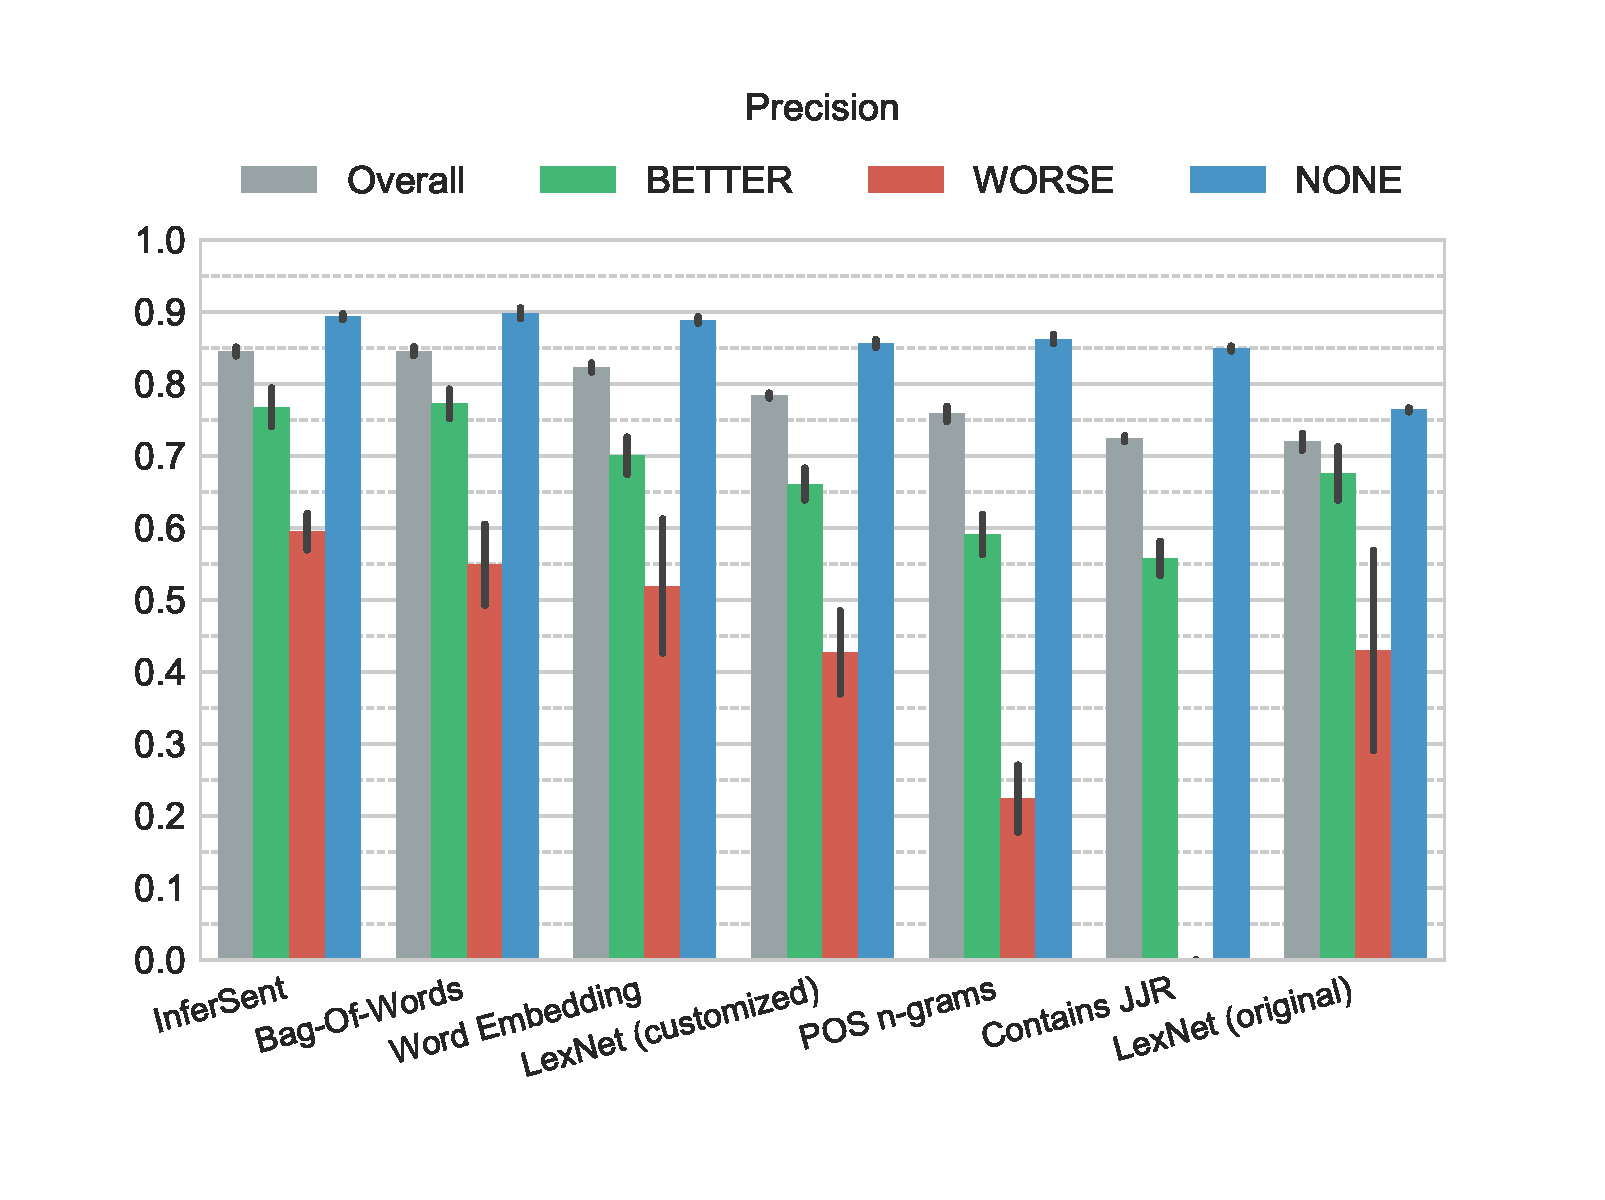
\includegraphics[scale=0.31,trim={2cm 0 0 0},clip]{images/experiments/p-precision-False}}
            \column{2in}
            \centerline{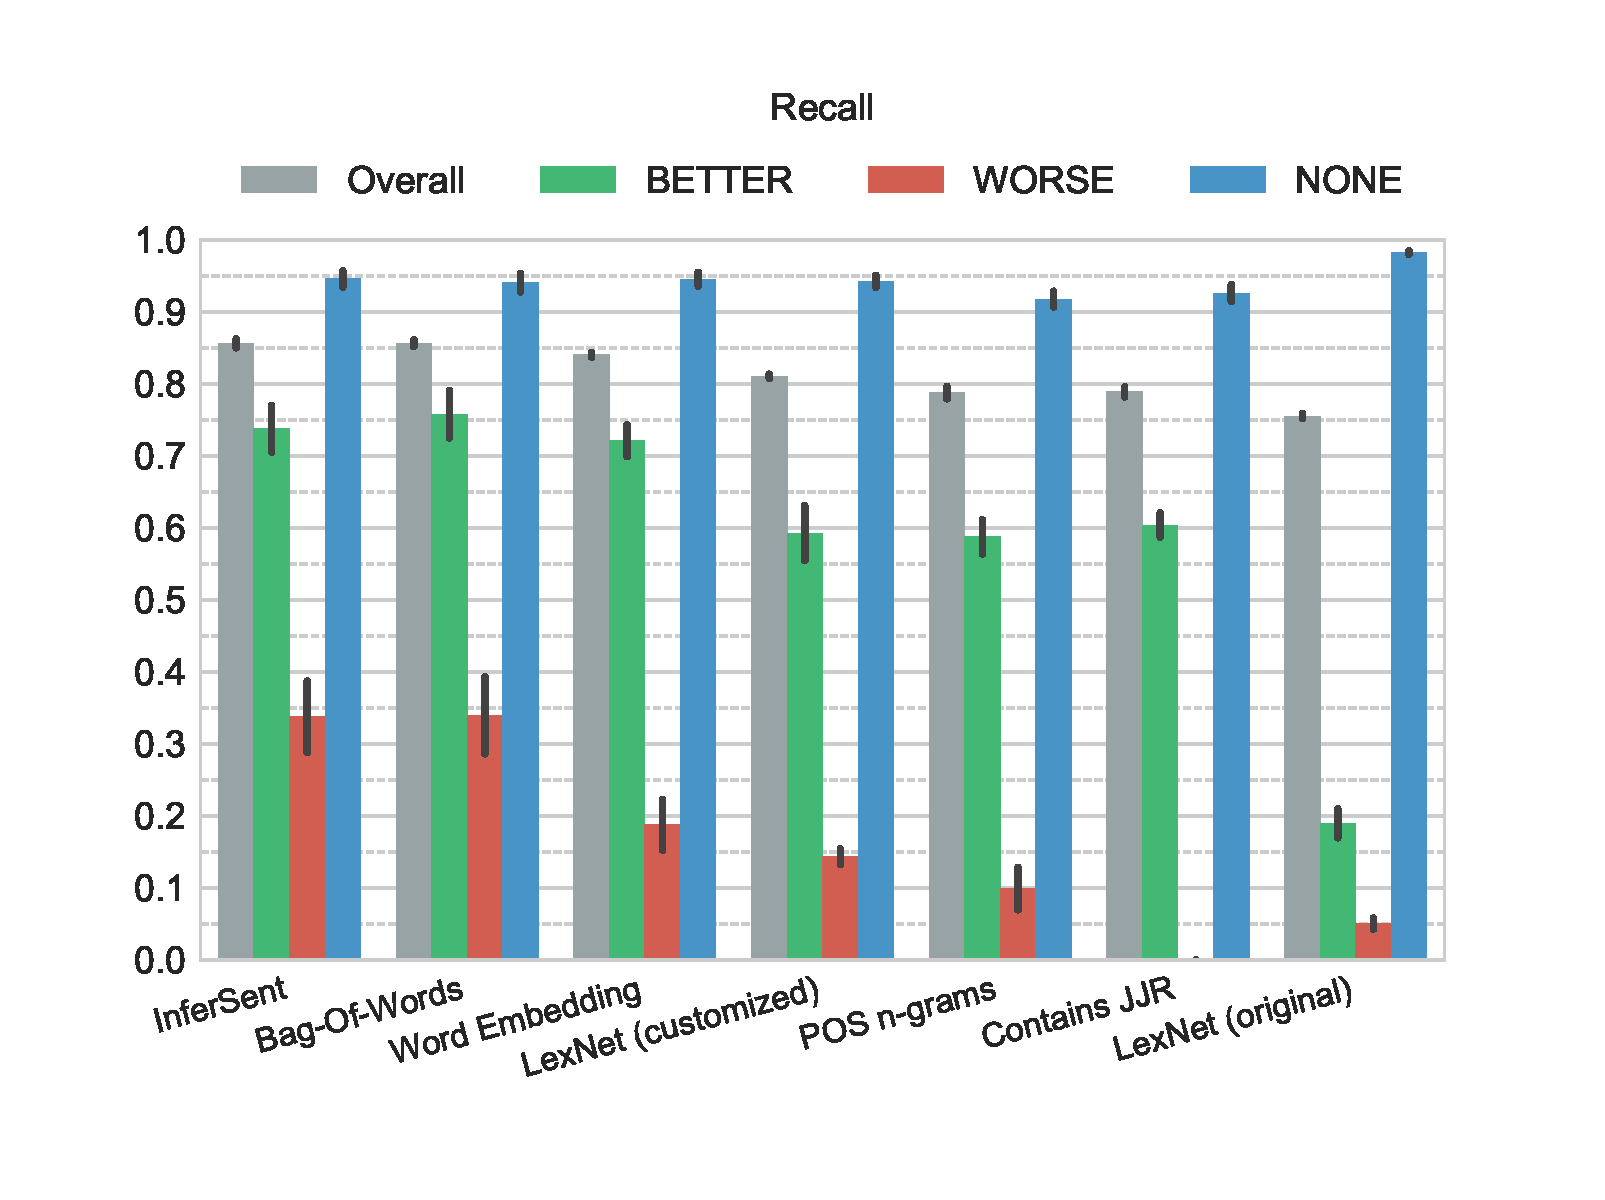
\includegraphics[scale=0.31,trim={0 0 2cm 0},clip]{images/experiments/p-recall-False}}

        \end{columns}
    \end{frame}

    \begin{frame}[t]
        \frametitle{Binary: F1 score}
        \centerline{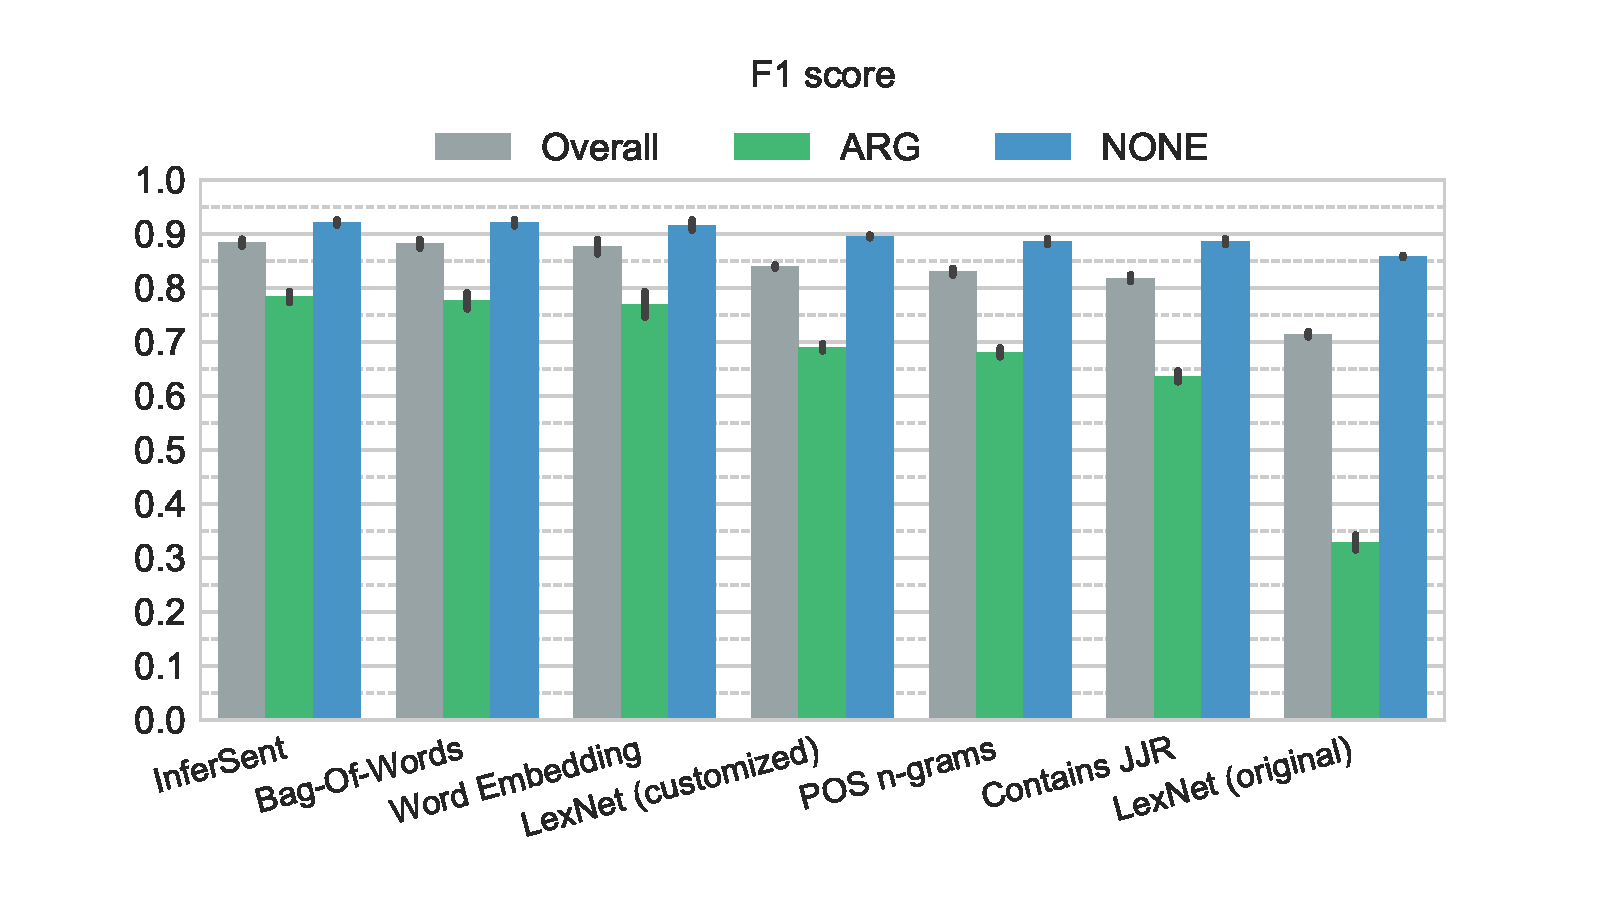
\includegraphics[scale=0.45,trim={0 0 0 0.5cm},clip]{images/experiments/p-f1-True}}
    \end{frame}


    \begin{frame}[t]
        \frametitle{Binary: Precision and Recall}
        \begin{columns}[t]
            \column{2in}
            \centerline{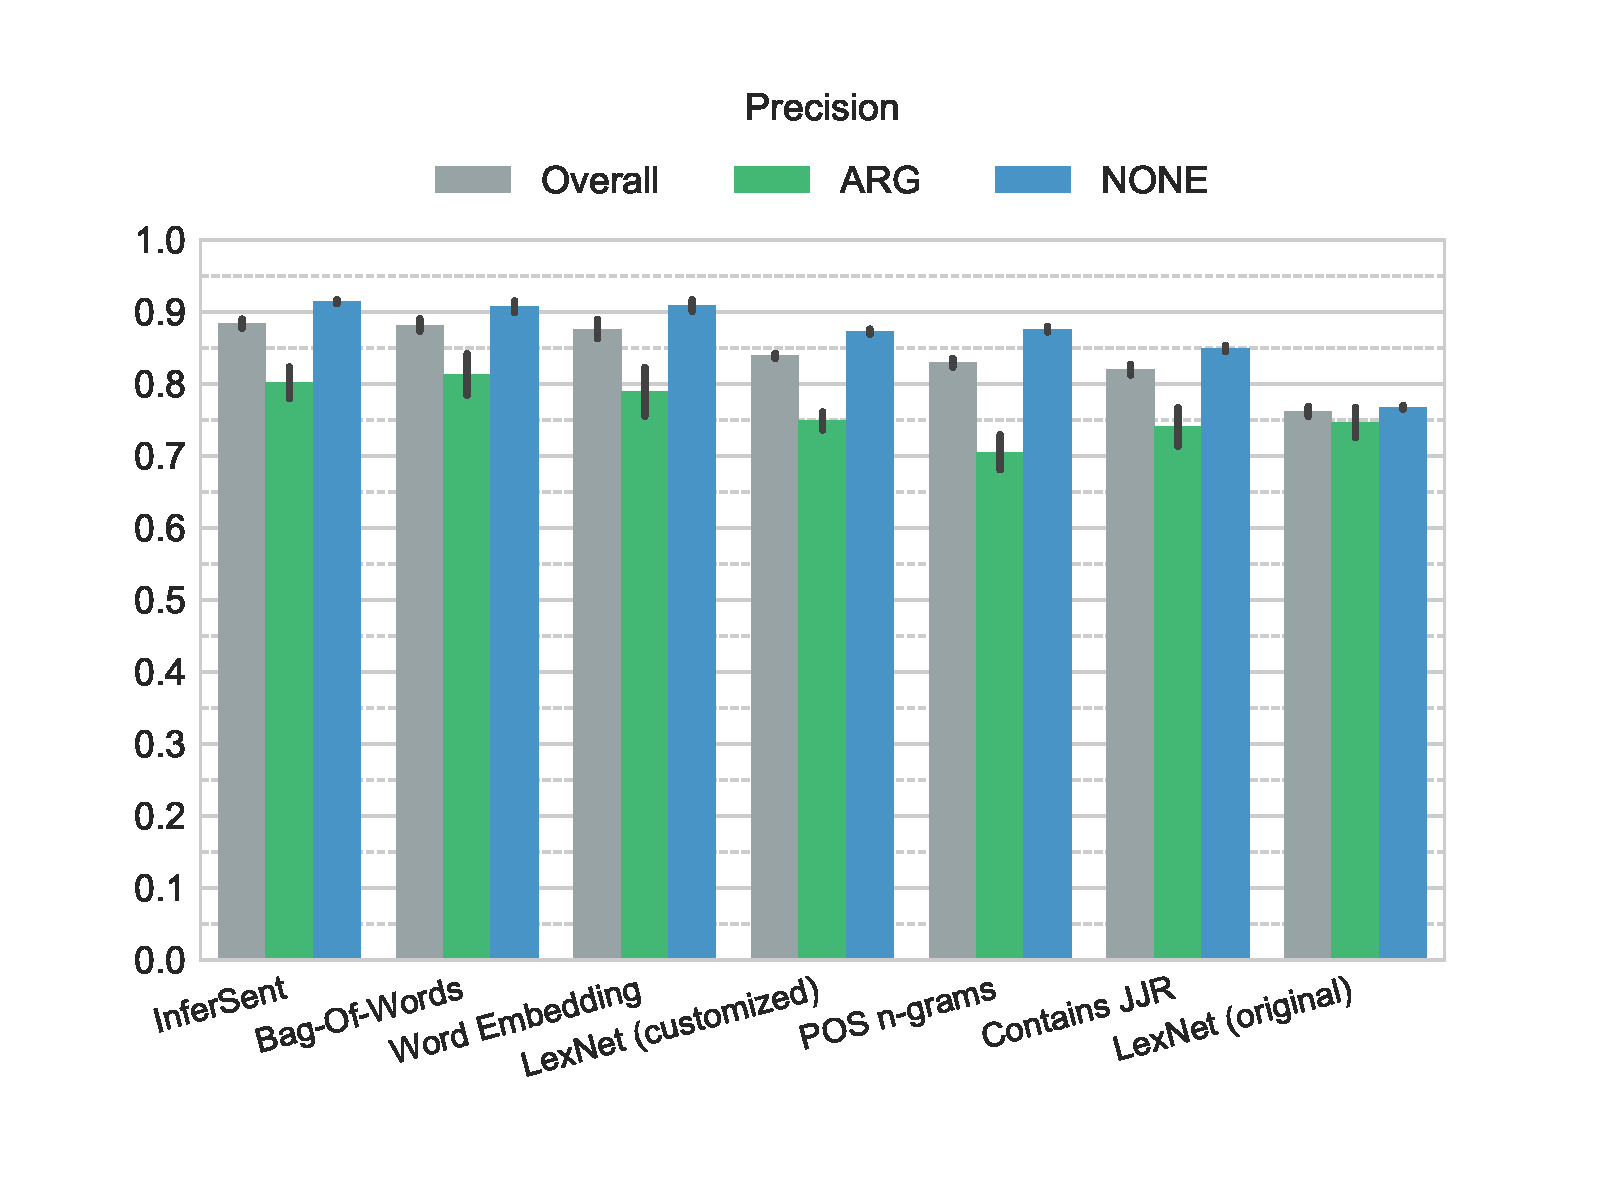
\includegraphics[scale=0.31,trim={2cm 0 0 0},clip]{images/experiments/p-precision-True}}
            \column{2in}
            \centerline{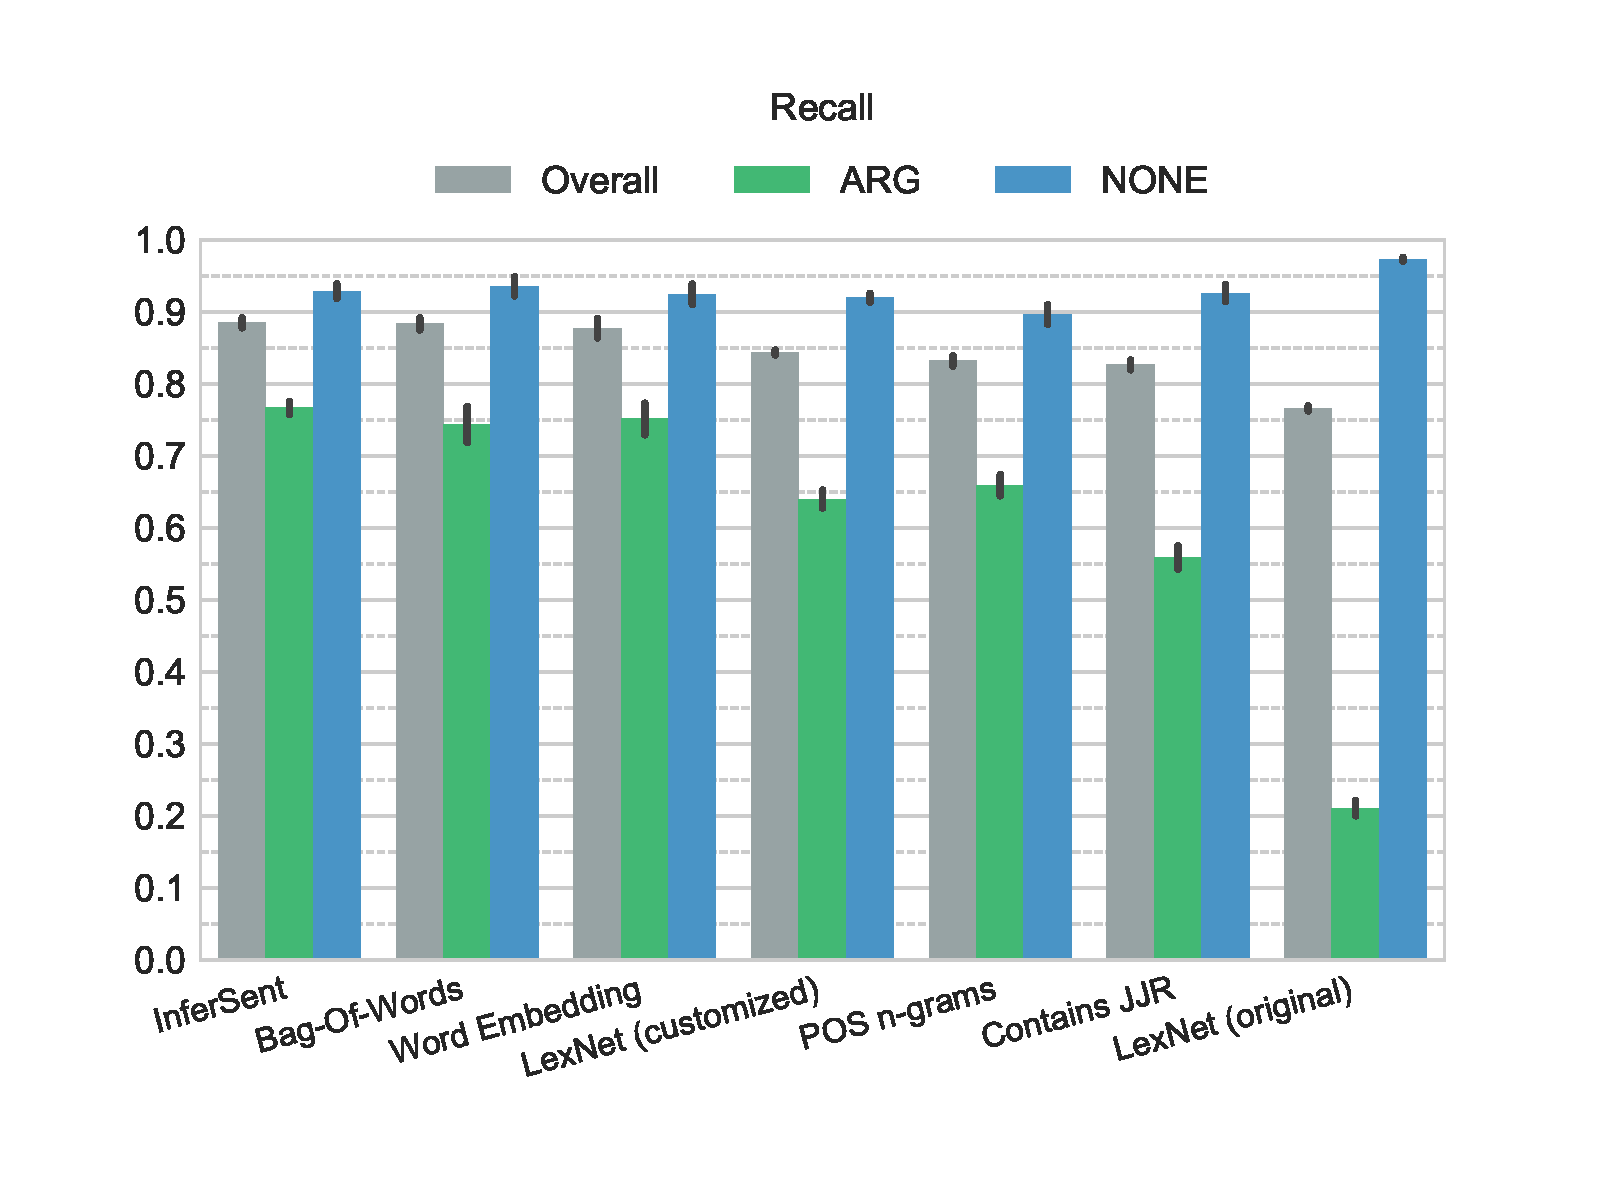
\includegraphics[scale=0.31,trim={0 0 2cm 0},clip]{images/experiments/p-recall-True}}

        \end{columns}
    \end{frame}

    \begin{frame}[t]
        \frametitle{Intermediate Results}
        \begin{itemize}
            \item As expected, \texttt{WORSE} is hard to recognize.
            \item InferSent, Bag-Of-Words and Mean Word Embeddings have a similar f1 score
            \item InferSent is more precise on \texttt{WORSE}.\pause
            \item The best f1 score is 24 points above the baseline.
            \item The original LexNet setup is the worst, but still above the baseline.
            \item The binary scenario is only slightly better than the three class scenario.\pause
            \item Using only the middle part of the sentence \textbf{increases the f1 score by 6-13 points}.
            \item The objects contribute only little to the result; removing or replacing did not alter the f1 score by more than 0.005 points.
        \end{itemize}
    \end{frame}

    \subsection{Error analysis}
    \begin{frame}[t]
        \frametitle{Error Analysis 1}
        Errors made by InferSent and LexNet (optimized)
        \begin{itemize}
            \item<1> 1311 sentences were incorrectly classified (three class scenario).
            \item<1> 607 errors were made by both features.
            \item<1> 220 additional were exclusively made by InferSent, 484 by LexNet.
            \item<1> the errors made in the binary scenario are similar (1183 errors, 739 shared with the three-class scenario, 444 new).
           
        \end{itemize}

    \end{frame}
    
    
    \begin{frame}[t]
        \frametitle{Error Analysis 2}
        
        \begin{itemize}
         \item The majority of errors was made on sentences with a high annotation confidence.
            \item Identified problems:
            \begin{itemize}
            \item questions
            \item negations
            \item missing cue words
            \item comparative sentences which do not compare the objects
            \item missing context / knowledge
            \end{itemize}
            \item \texttt{WORSE} was confused with \texttt{NONE} more often than with \texttt{BETTER}
        \end{itemize}

        \end{frame}

    %=========== HELD OUT HELD OUT
    \subsection{Evaluation with the Held-Out Data}
    \frame{\subsectionpage}

    \begin{frame}[t]
        \frametitle{Three classes: F1 score}
        \centerline{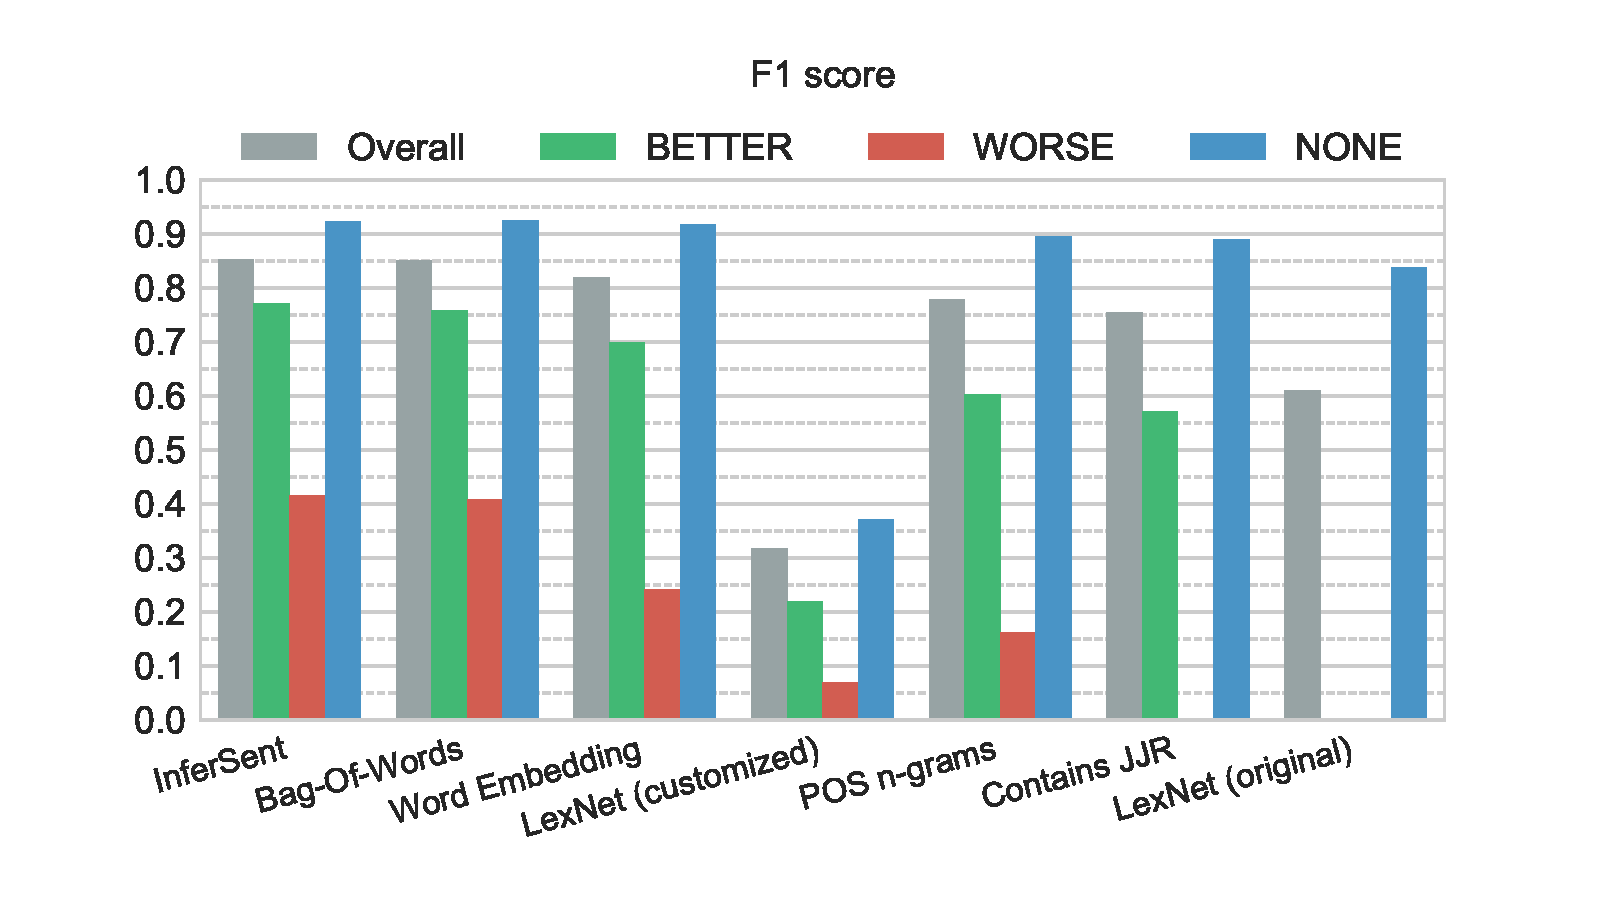
\includegraphics[scale=0.45,trim={0 0 0 0.5cm},clip]{images/experiments/hp-f1-False}}
    \end{frame}


    \begin{frame}[t]
        \frametitle{Three classes: Precision and Recall}
        \begin{columns}[t]
            \column{2in}
            \centerline{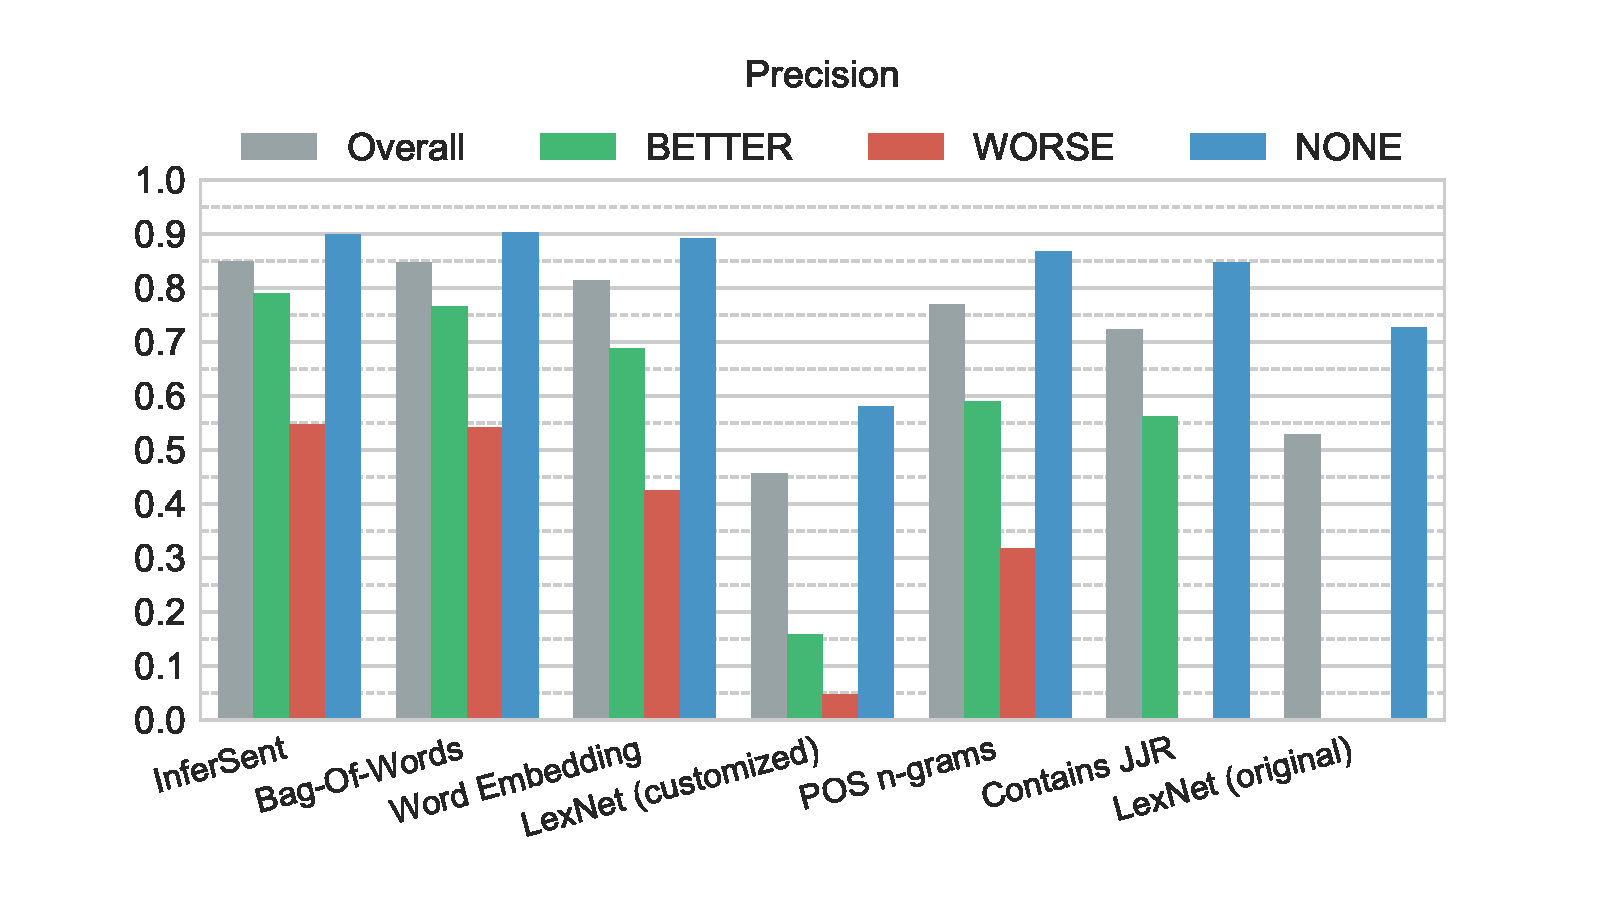
\includegraphics[scale=0.31,trim={2cm 0 0 0},clip]{images/experiments/hp-precision-False}}
            \column{2in}
            \centerline{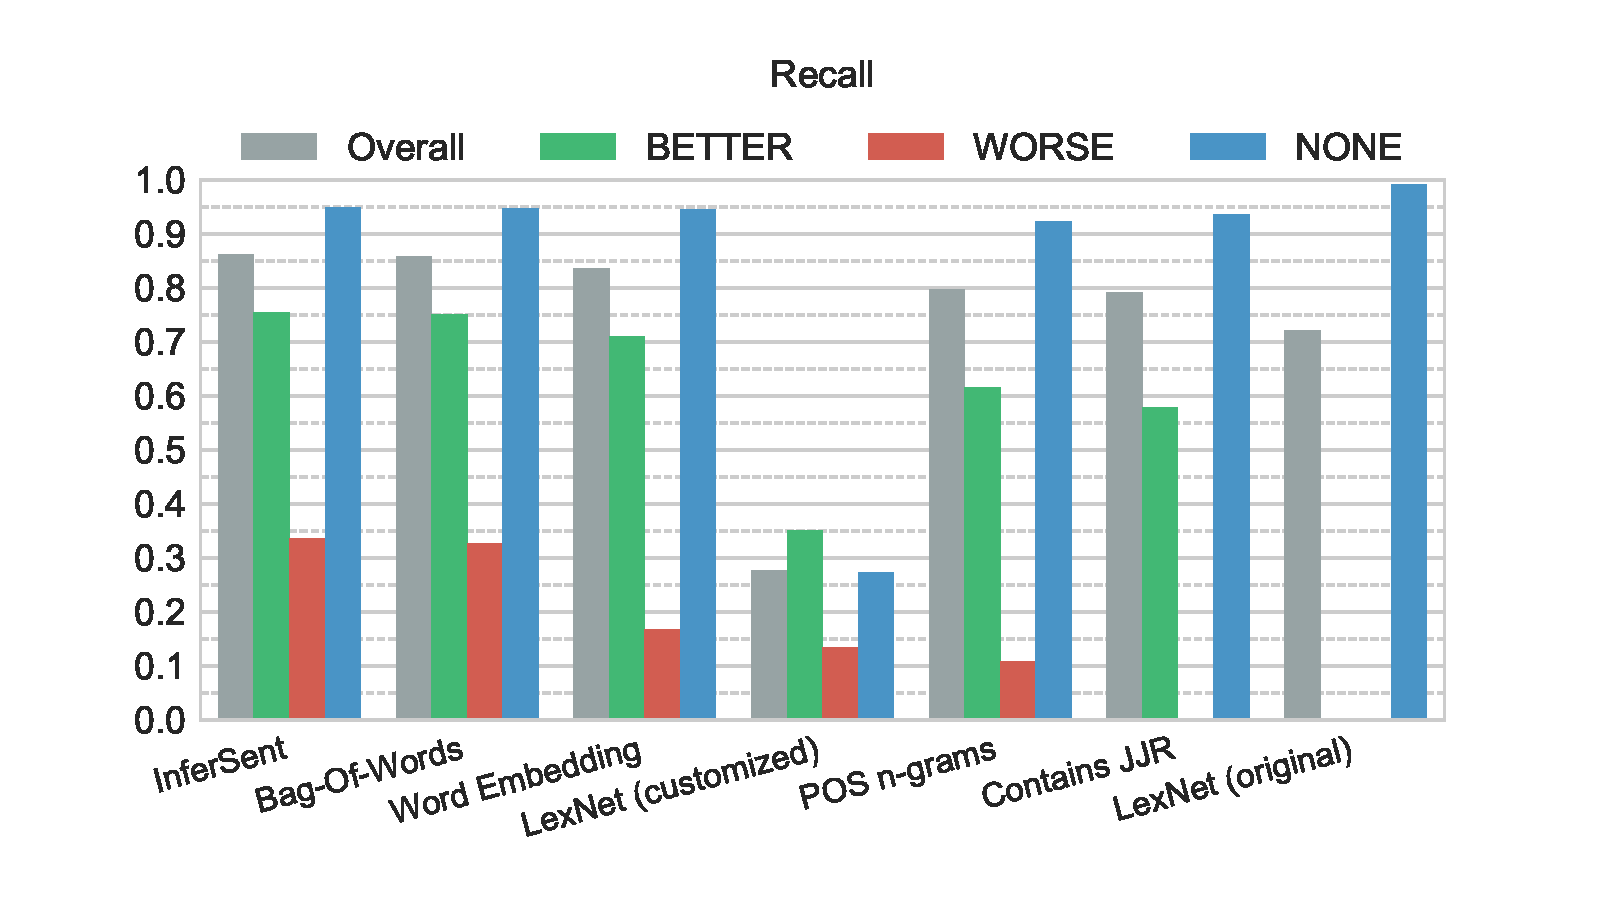
\includegraphics[scale=0.31,trim={0 0 2cm 0},clip]{images/experiments/hp-recall-False}}

        \end{columns}
    \end{frame}

    \begin{frame}[t]
        \frametitle{Binary: F1 score}
        \centerline{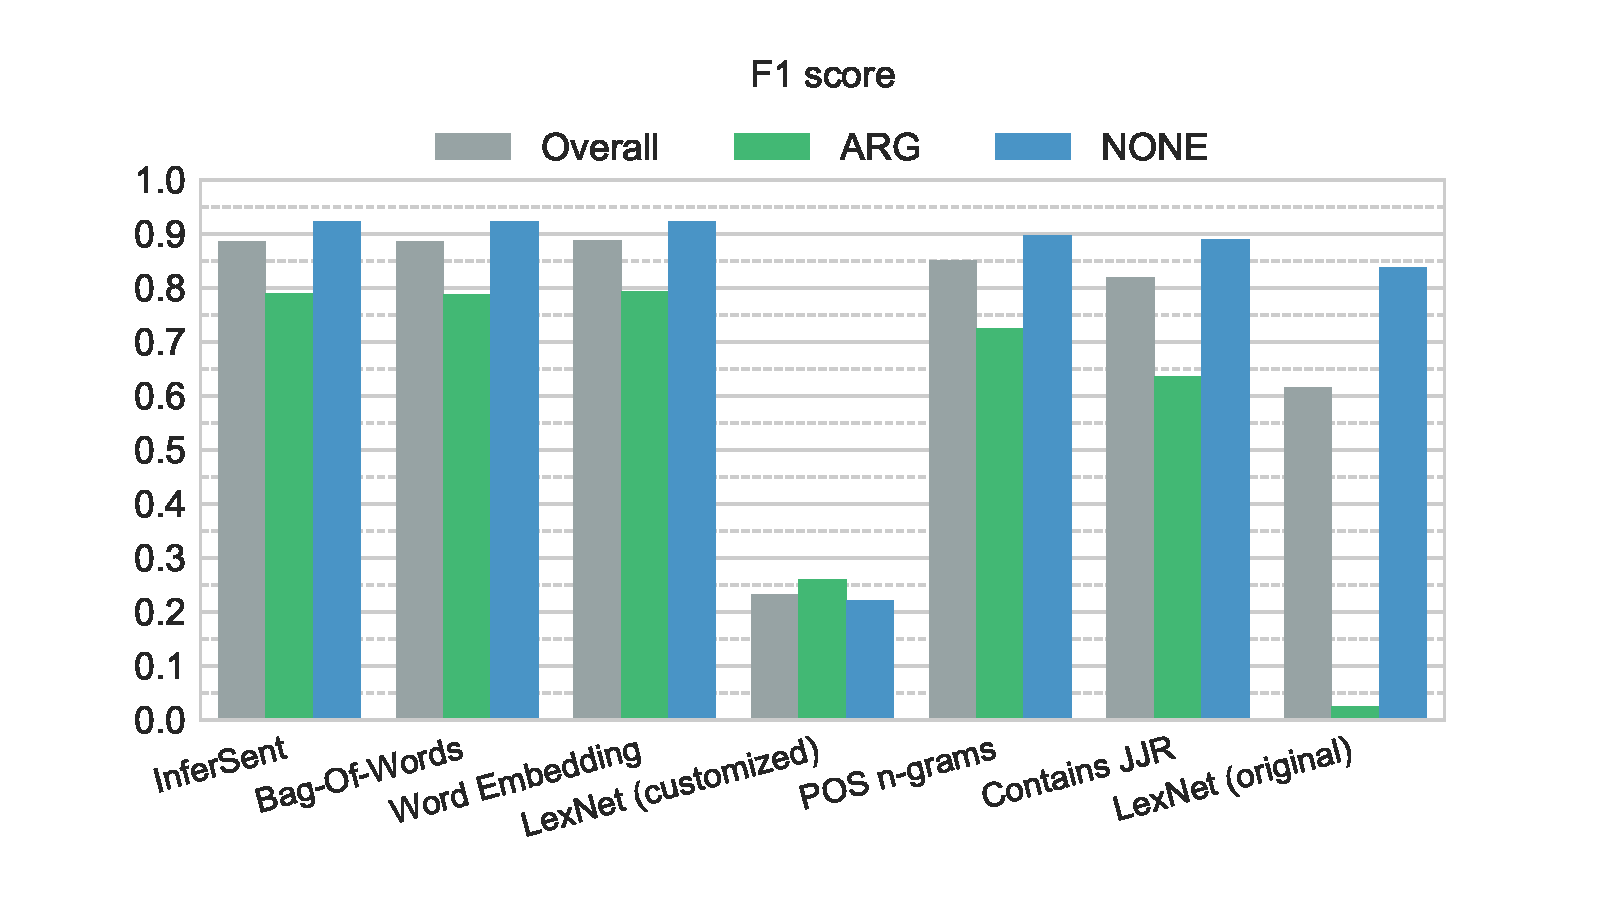
\includegraphics[scale=0.45,trim={0 0 0 0.5cm},clip]{images/experiments/hp-f1-True}}
    \end{frame}


    \begin{frame}[t]
        \frametitle{Binary: Precision and Recall}
        \begin{columns}[t]
            \column{2in}
            \centerline{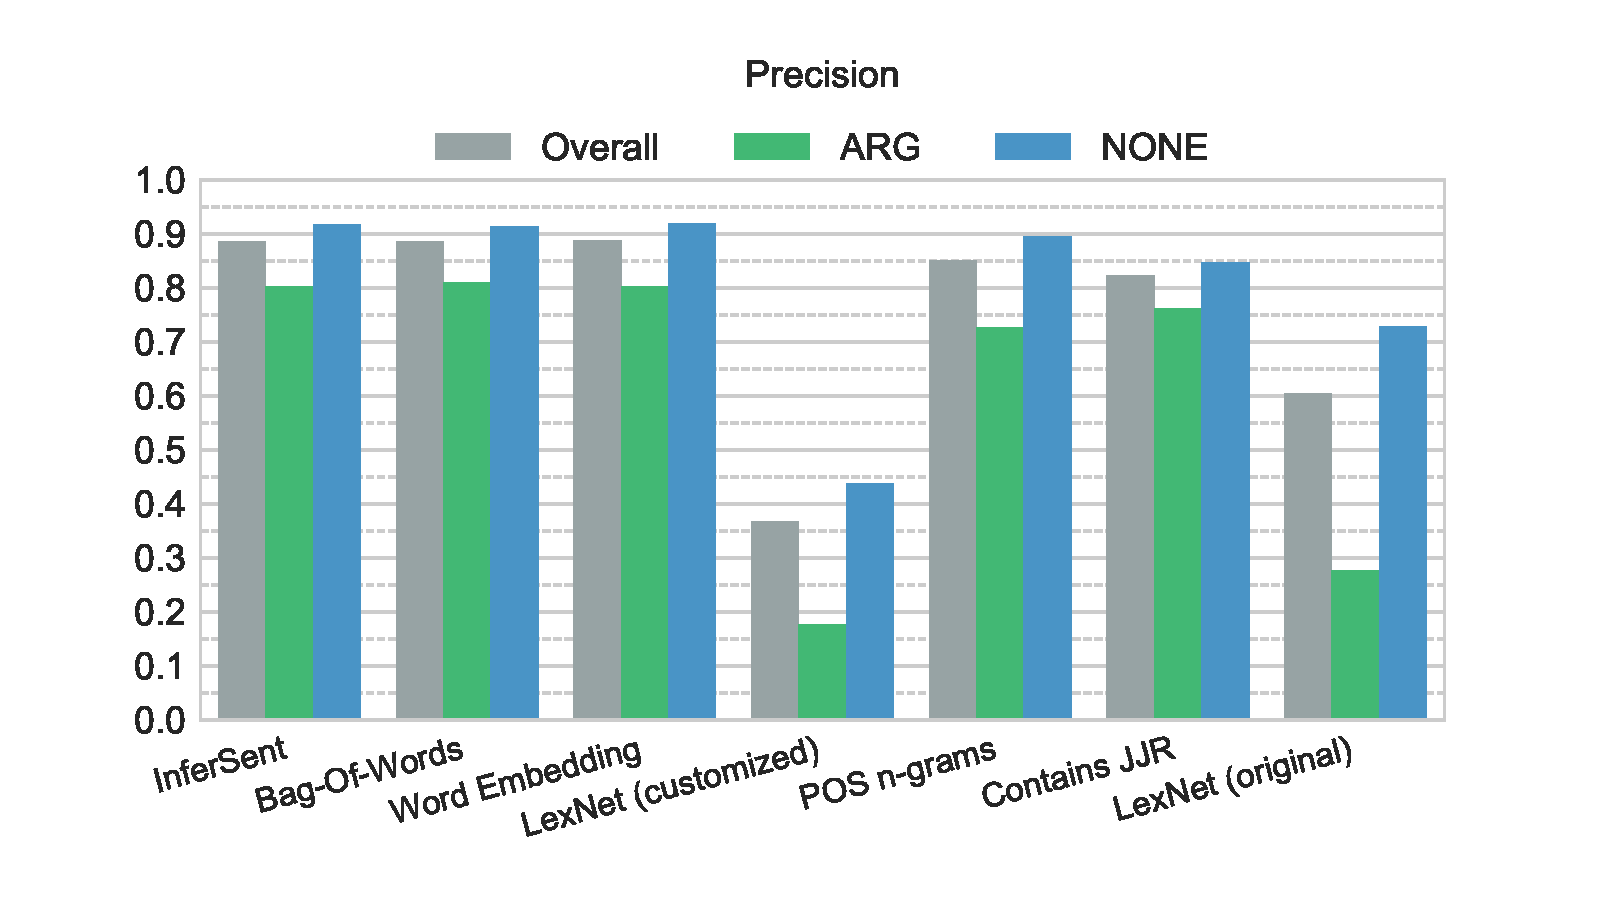
\includegraphics[scale=0.31,trim={2cm 0 0 0},clip]{images/experiments/hp-precision-True}}
            \column{2in}
            \centerline{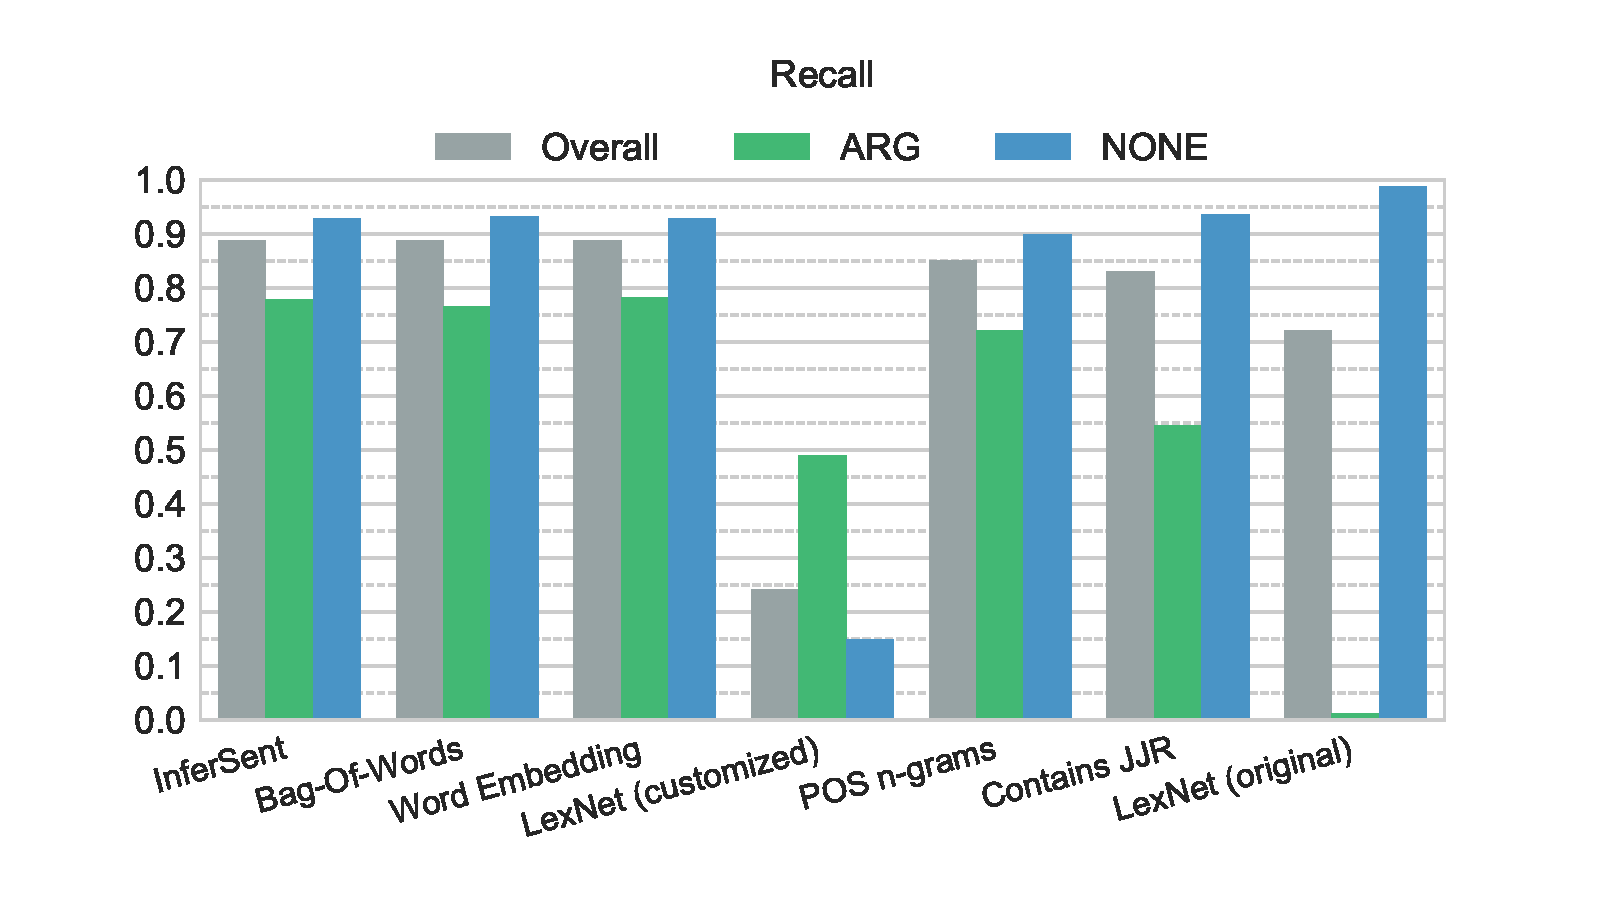
\includegraphics[scale=0.31,trim={0 0 2cm 0},clip]{images/experiments/hp-recall-True}}

        \end{columns}
    \end{frame}

    \begin{frame}[t]
        \frametitle{Results}
        \begin{itemize}
            \item InferSent is the best feature.
            \item The LexNet feature did not generalize:\pause
            \begin{itemize}
                \item 2344 unique paths for 5759 sentences (training set)
                \item 594 unique paths for 1441 sentences (held out set)
                \item training and held had only 81 paths in common
            \end{itemize}
            \item No feature combination was better than InferSent.
        \end{itemize}
    \end{frame}

    \section{Conclusion and Future Work}
    \frame{\sectionpage}
    \subsection{Conclusion}
    \begin{frame}[t]
        \frametitle{Conclusion}
        \begin{itemize}
        \item The best feature could yield an f1 score of 0.85; 24 points \textbf{above} the baseline.
        \item Simple features (bag-of-words) perform almost equal to more complex features.
        \item HypeNet needs way more training data!\pause
        \item Objects are not important for the classification at all.
        \item Preprocessing is crucial to achieve good scores.\pause
        \item Contrary to the expectations \texttt{WORSE} is more similar to \texttt{NONE} than to \texttt{BETTER}.
        \item All in all, the crowd sourcing and classification worked satisfactorily.
        \end{itemize}
    \end{frame}
      \subsection{Future work}
    \begin{frame}
        \begin{itemize}
        \frametitle{Future work}
    \item More data!
    \item Add more features to capture special case, for instance questions
    \item Use surrounding sentences for context information and coreference resolution
    \item Test in a real world application
    \end{itemize}
    \end{frame}



    \begin{frame}[allowframebreaks]
        \frametitle{References}
        \bibliographystyle{apalike}
        \bibliography{main}
    \end{frame}
    
    \begin{frame}
    \begin{center}
    \begin{LARGE} Thank you! Questions? \end{LARGE}\\\par
    \hfill \\
    franzek@posteo.net
    \end{center}

    \end{frame}

\end{document}